\documentclass[11pt]{article}
\usepackage[english]{babel}
\usepackage{geometry}

\usepackage{booktabs}\newcommand{\ra}[1]{\renewcommand{\arraystretch}{#1}}

%bibliography packages
\usepackage{natbib}
\usepackage{booktabs}
\usepackage{amssymb}
\usepackage{tabularx}

\usepackage{multicol, caption}
\usepackage{wrapfig}
\usepackage{float}
\usepackage{hyperref}


\title{\vspace{-2.0cm} \textbf{Tracing Swiss National Identity in Regional Newspapers across the XIX and XX Century}}
\author{by Aurel Maeder, Ludovica Schaerf, Michal Bien}
\date{}

\usepackage{natbib}

\usepackage{graphicx}
\usepackage{array, makecell} 
\usepackage{amsmath}
\usepackage{amssymb}% http://ctan.org/pkg/amssymb
\usepackage{pifont}% http://ctan.org/pkg/pifont
\newcommand{\cmark}{\ding{51}}%
\newcommand{\xmark}{\ding{55}}%

\usepackage{caption}
%\captionsetup[figure]{font=tiny}

\begin{document}




\maketitle

\section{Introduction}

The XIX century in Europe is, among others, defined by the emergence of the nation state as exemplified by the German (1871), Italian (1870) and Swiss nation (1848). Whereas the French, English, German or Italian nations emerged either from a preceding dynastic power over a given geographic territory or a common language, ethnicity and culture  \footnote{"Tantôt l'unité a été réalisée par une dynastie, comme c'est le cas pour la France ; tantôt elle l'a été par la volonté  directe  des  provinces,  comme  c'est  le  cas  pour  la  Hollande,  la Suisse,  la  Belgique ;  tantôt  par  un  esprit  général,  tardivement  vainqueur des  caprices  de  la  féodalité,  comme  c'est  le  cas  pour  l'Italie  et  l'Allema-gne." \citep{renan1882qu}}, Switzerland constitutes a special case\footnote{"Comment  la  Suisse,  qui  a  trois  langues,  deux  religions,  trois  ou  quatre races, est-elle une nation" \citep{renan1882qu}}. \par
For most of its history, Switzerland was a loose federation of different city-states or small independent regions bound together by a military entity called the Swiss confederation. Thus, Swiss people preferably identified with their local region, canton, or even city than with the Swiss confederation for a long time. \par
However, during the last two centuries, a Swiss identity arguably emerged, aided by shared military service, education, historical education, and common values. This “growing together” was also manifested in the growth in central authority (implementation of national pension schemes and inter-cantonal transfers; \cite{ladner2018schweizer}). \par
Due to their exceptional stance, Swiss nationalism and national identity have been discussed by a rich body of literature from different scientific communities. 
In our analysis, we would like to contribute to this general discussion by tracing the evolution of Swiss national identity from the XIX century using computational methods. Specifically, we consider the period from the 1820s to the 1950s, when the formation and development of the modern Swiss Nation took place. This analysis aims to articulate the concept of Swiss nationality in a computer-understandable manner and to scan the vast corpus of regional Swiss newspapers for its evolution in time. Newspapers have been chosen as, we believe, they largely reflect and model the opinions and topics of interest to the regional population. To the best of our knowledge, the adoption of newspapers as a primary source has not yet been considered in the analysis of Swiss nationality and could hopefully provide new insights into the matter. \par
The investigation will comprise two parts: the extraction of expressions that identify Swiss identity and the temporal evolution of how these expressions were used in the selected newspapers. For the extraction, we adopt several textual sources that can serve as proxies of national identity. Those proxies are: 1) Early Swiss history books. 2) World War I propaganda articles in newspapers. 3) Political sociology papers on (Swiss) nationalism. Although all presented proxies are inherently biased, by looking at the question from several angles and taking different proxies into account, this paper aims to produce meaningful and robust results. 

\section{Context}

This section presents the historical and sociological discussion surrounding the exceptional case of the Swiss nation and the Swiss identity, which motivates this project and its Methodology. Furthermore, the presented sources carry different definitions of Swiss identity and can thus be used to extract meaningful terms, which define Swiss identity throughout the century. In practice, this project uses two history books\footnote{\cite{MuellerJohannes1780} and \cite{seippel1900schweiz}}, World War I propaganda articles published in Swiss newspapers available in Impresso platform, and several sociological papers which deal with Swiss identity to extract 'Swiss identity terms' as it will be described in the Methodology.  


\subsection{Swiss History}

The modern Swiss nation arguably emerged from a complex construct of treaties and inter-regional dependencies commonly referred to as the 'Swiss Confederation' \citep{Eidgenossenschaft_hsl_2012}. The members of this confederation were bound together by a multitude of contracts \footnote{The oldest still existing contract dates back to 1291}. \citep{Bundesbriefe_hsl_2012}.\par
Those medieval contracts and treaties often resisted the influence of surrounding European powers (especially France and the Hapsburg) while reinforcing economic links between the Swiss regions. 
Early historians would reinterpret those early contracts between the members of the Swiss confederation as a shared endeavor for self-government, autarchy, and self-determination of the individual Swiss regions (see 'Chronicon Helveticum' \cite{tschudi1734chronicon}.\par
In the 18th century, nationalistic forces driven by the spirit of the enlightenment used a similar narrative to solidify their case for a unified Swiss nation. Extending on it by claiming that the Swiss people must be considered a homogeneous ethnicity\footnote{The so-called 'helvetics', populating the central alps} and thus belong in a common nation (see 'The history of the Swiss confederates' \cite{MuellerJohannes1780}. \par
This ethnic understanding of the Swiss nation was deeply questioned at the end of the 19th century.
Historians increasingly argued that the concept of 'the Swiss nation and its people' was created during the 19th century aided by national institutions as standard military service, national celebrations, national societies, and a common myth of origin (see \cite{seippel1900schweiz} and \cite{renan1882qu}). \par


The two world wars asserted again the importance of a common Swiss national identity. During this time, the central government and military leadership allocated considerable resources to solidify Swiss patriotism, in an act which would be referred to as 'spiritual defense'. This ideology stated that Switzerland in its cultural and ethnic diversity was unified by a common set of beliefs and a 'spiritual unity'\footnote{"L'idée  suisse  n'est  pas  un  produit  dela  race,  c'est-à-dire  de  la  chair,  mais  une  œuvre de  l'esprit.  C'est  un  faitadmirable  qu'autour  du  Gothard,  montagne  qui  sépare  et  col  qui  unit,une grande idée,  une idée européenne, universelle, ait  pu prendre naissanceet  devenir  une  réalité  politique:  l'idée  d'une  communauté  spirituelle  despeuples  et  des  cultures  occidentales." (P. 1012, \cite{conseilFederal1938})}. \citep{LandesverteidigungJorio_hsl_2012} \par 
In practice, for extracting Swiss identity from Swiss history books, the works of \cite{MuellerJohannes1780} and \cite{seippel1900schweiz} in French and German language have been used. 

\subsection{Political Sociology of Nation}
Many influential authors addressed the 'Swiss case' as that edge case that could confirm or dismiss their theory on nationhood. Among others, the names Anderson, Renan, Weber, Kohn appear in the long list (\cite{wimmer2011swiss}). 
\par

According to \cite{wimmer2011swiss}, Switzerland is a case of a multi-ethnic nation, where even cantonal borders are independent of language borders. However, even considering Switzerland multi-ethnic has been widely questioned, and numerous other options have been put forward. Switzerland has been considered post-national, multi-national, quasi-ethnic, and much more \citep{helbling2011switzerland}. Alongside the problematization of its definition as a nation, \cite{wimmer2011swiss} and \cite{helbling2011switzerland} show how major theorists differ widely in their explanation on the nature and foundation of Swiss nationality: Weber \footnote{\citep{weber1978economy}} sees Switzerland as an example of how a nation can be based on the commonality of political spirit rather than objective attributes. For Kohn \footnote{\citep{kohn1956nationalism}} and Deutsch \footnote{\citep{deutsch1953nationalism}}, the republican regime and the advanced communication channel created the cohesion of this nation despite its lack of common cultural background. Gellner \footnote{\citep{gellner1991nationalisme}, \citep{gellner2008nations}} argues that the Swiss nation can only be explained taking into account the extremely high level of literacy, which removes the need for a shared language. 
Based on the above theories, \cite{wimmer2011swiss} identifies the creation of the Swiss national concept in the bourgeois associations that formed in the XVII century. These associations aimed at a progressive union and equality between rural and urban areas. Those societies proclaimed a 'community of progress' that was meant to disseminate the national sentiment, based on republican and liberal ideals rather than nationalism itself.

Overall, the Swiss case can be well explained as a process shaped by a changing social context, where the will of the people (Willensnation) and the natural communion of the different ethnicities (Wesensgeheimschaft) forged Switzerland as a nation \citep{zimmer1999forging}. The first entails a political action, where some key actors form the Swiss concept of nation and the population follows. The second is the ensemble of pre-existing indigenous folk traditions, myths, symbols, narratives, and
beliefs, which distinguish the Swiss from the outside \citep{zimmer1999forging}. \par

Lastly, it is necessary to keep in mind the critical accounts given by Anderson and Renan. The first envisages nation as "an imagined political community [...] It is imagined because the members [...] will never know most of their fellow-members [...], yet in the minds of each lives the image of their communion (p.2)" \citep{anderson2006imagined}. Switzerland is, therefore, a nation in virtue of the imagination of its members to belong to the same nation. According to \cite{renan1882qu}, the nation is a "spiritual principle" based on a shared past and heritage. In line with this theory, the Swiss proclaim themselves Swiss given their common past.
\par
To create the corpus for extraction, the papers cited by \cite{wimmer2011swiss} and \cite{helbling2011switzerland} and written in either French or German were searched for (i.e. \cite{imhof1993nationalismus}). Since not all of those were publicly available, papers citing the major theorists were also downloaded whenever possible (i.e., \cite{godechot1971nation}). Attention was paid to retrieving older, foundational papers (from the 1960s-1990s) and more recent ones (XXI century). Moreover, both papers discussing specifically the Swiss case and those introducing a general theory of nationalism were included. Finally, texts about different theories (subjectivist, objectivist, ...) were retrieved. The full list of papers gathered can be found in Appendix 1. 

\section{Data}

For the analysis, data are used for two purposes: extracting expressions on Swiss identity and tracing the expressions in newspapers. Regarding the first use, the three types of sources were already mentioned in the Research Context. The texts mentioned are retrieved in .txt format, and they consist of two history books, newspapers containing propaganda, and 18 political sociology papers. Most of these resources are retrieved from the Swiss National Library, French National Library (Gallica), Google Books, and E-Periodica. \par

Each of the three types of sources is associated with a reference corpus to extract TF-IDF scores by computing an inverse document frequency. For the three corpora, texts with similar language to the original corpus but a different content are searched. A suitable reference corpus for Swiss historical literature in French and German is provided in the 'Trés Grand Bibliotheque' \citep{TresGrandBibliotheque} and the 'Deutsches Textarchiv'\citep{DeutscheTextArchive}. For WW1 propaganda newspapers, a sample of 10000 articles from the Swiss press, published in the two major newspapers in the period before WW1 (1901-1914) serves as a reference, assuming there was no need for national propaganda before the war had started. For sociology articles, a corpus of papers published in JSTOR sociology journals between 1960-2020 in French (and containing the word sociologie) and German (and containing the word Soziologie) is used. \par

In terms of the second use, this project adopts a large-scale corpus of different regional newspapers, the Impresso Platform, by \cite{Ehrmann2020LanguageRF}. The Impresso project gathered and pre-processed an impressive corpus of over 36 million articles from a diverse set of Swiss newspapers. To our best knowledge, it is the largest data set that can be easily used to analyze Swiss newspapers over the XIX and XX centuries. An exploratory analysis has shown that a reasonable amount of data is available in two out of the four Swiss national languages: French and German.\par
Finally, only the Gazette de Lausanne and Neue Zuricher Zeitung were used as these are two local newspapers representative of their regions, issued in the capitals of the cantons with the biggest french-speaking and german-speaking population. 


\section{Methods}
As for the Data, the Methodology comprises two steps: a TF-IDF n-gram extraction from the corpora on Swiss identity and a longitudinal analysis of the frequency of the extracted unigrams over the two selected journals in the Impresso Platform. \par

From the three corpora gathered (as described in the sections above), pre-processing steps were applied to obtain a clear extraction: the texts were tokenized, stopwords were removed, and POS (Part of Speech) tagging was used to maintain only adjectives, adverbs, nouns, pronouns, and verbs (as we consider those the most informative parts of a sentence). Furthermore, lemmatization was used to reduce terms to their word stem.\par
Following, the TF-IDF scores were computed for 1-grams to 4-grams, where the inverse term frequencies were computed against reference corpora, and the resulting weights for each word were determined as follows:
\[w_{i,j} = tf_{i,j} \cdot log(\frac{N}{df_{i}})\]
where $w_{i,j}$ is weight of the word $i$ in document $j$, the $tf_{i,j}$ is the number of occurrences of $i$ in $j$, $N$ is the number of documents and $df_{i}$ is the number of documents containing the word $i$. \par

Each type of source was considered as one document and compared against all the documents in the corresponding baseline corpus. The 50 unigrams with the highest resulting weights for each type of source were then used in the n-gram frequency analyzer in the Impresso Platform\footnote{The tool can be found \href{https://impresso-project.ch/app/search/ngrams?sq=ChYIARACGAcgASoMbmF0aW9uYWxpc21l}{here}}. The previous work of \cite{Twenge2012IncreasesII} shows that the quantitative analysis of the word frequency in time on the large corpora can unveil the trends, not only in language but also in the changing society and public opinions. With this purpose in mind, this project uses the extracted words to show how their aggregated yearly trends of use fluctuated through time. Once the words are plugged in, the tool scans through all the OCRed corpus and calculates the aggregated frequency in time for the selected n-grams, in absolute values, and as a ratio per million tokens. Some filtering is applied before the search: only articles in French and German published in Switzerland in Gazette de Lausanne, or Neue Zuricher Zeitung were selected.  

Finally, the frequency per million tokens of the 50 unigrams is aggregated and plotted in time with a running mean of a decade. The resulting plots can be observed in the Results section. 

\section{Results}
\subsection{History}
By using the historical works of \cite{MuellerJohannes1780} and \cite{seippel1900schweiz} and comparing them with the aforementioned reference corpora with the TFIDF method, we obtain the term list presented in Appendix \ref{appendix4}. \par
\begin{table}[H]
\small
\begin{scriptsize}
\centering
\caption{Selected terms, Swiss history}\label{TFIDF_Terms_Top_Twenty_desc}
\hspace*{-1.5cm}
\begin{tabular}{|l|l|l|} 
\hline
Self identified Topic & German terms & French  terms  \\
\hline
\makecell{Swiss places  \\ or nation} & \makecell{zürich  / luzern / bern /  waadt / z̈urich bern / schweiz  \\ eidgenossenschaft / helvetien / helvetischen republik } & \makecell{berne /  zurich / bernois / schwyz  \\ suisse allemand  / suisse /  alliance }  \\
\hline
\makecell{Significant people in \\ Swiss history} & \makecell{numa droz  / bonaparte / general bachmann  } & \makecell{comte pierre /  rodolphe habsbourg / abbé saint-gall \\ empereur fŕed́eric /  jean bubenberge } \\
\hline
European powers   & \makecell{französisch  / frankreich / franz̈osisch gesandte \\ schweiz frankreich / franz̈osisch truppe } & \makecell{habsbourg /  empereur / savoie / maison habsbourg \\ empereur fŕed́eric  / habsbourg lauffenbourg }  \\
\hline
\makecell{Political institutions} & \makecell{tagsatzung / partei / behörde / verfassung \\ bürger / öffentlich / republik / volk \\ öffentliche meinung / volks nah \\ demokratischer kanton / neutralität schweiz } & \makecell{ bourgeois / charte  / alliance / frère \\ bourgeois berne/ traité paix /  électeur mayence } \\
\hline

\hline
\end{tabular}
\hspace*{-1.5cm}
\end{scriptsize}
\end{table} 
Analyzing the obtained German and French terms, one can identify recurring themes expressed by a group of terms that seem to describe the same concepts. Many of those identifiable themes occur in the German as well as in the French term lists.  \par 
The first apparent and intuitive topic is that of Swiss cantons, cities, places, or the Swiss nation itself. This topic seems to be a relatively intuitive result due to the chosen TF-IDF method, given that the comparative corpora probably rarely contain books that discuss Switzerland or Swiss cities. The three different terms used to name Switzerland (e.g., Schweiz, Eidgenossenschaft, Helvetik) correspond to names for Switzerland during different historical periods and already might imply the multifaceted nature of the Swiss identity throughout history. Furthermore, it is also interesting to analyze the cantons, cities, and places mentioned and, on the other hand, the places that are not mentioned. Here, one could state that the historical rivalry between and the importance of Bern and Zürich is visible given the high TF-IDF values of both cities and that there is even a bigram 'Zürich Bern'. \par
A similarly intuitive theme is the frequent mentioning of people, which might be significant for Swiss history. The most relevant bigram for the German list, for example, is the name Numa Droz, who was an influential Swiss politician and one of the first members of the federal council. The French list refers multiple times to Rodolphe Habsbourg, a medieval ruler who repeatedly waged war against the Swiss confederation. The French term list also mentions Whilhelm Tell (Guillaume Tell), who reportedly rebelled against the Habsburgs. \par
Another related and dominant theme visible in the term lists is that of foreign European powers. This theme might substantiate the fact that the surrounding European powers deeply influence the creation of the Swiss nation, as already discussed in the literature part. Interestingly, comparing the French to the German term list, it is notable that, while the French list mostly mentions the Habsburgs, the German term list instead mentions the French empire. This phenomenon is most probably the result of the different reference corpora, given that the French reference corpus is more likely the discuss French history, while the German reference corpus instead discusses the history of the German empires.  \par
A last notable theme discusses Swiss political institutions and principles. This topic is more ambiguous and mentions terms like the government, the constitution, the public, the people, the military, and neutrality. Although many of those words have a very strong connotation in discussing Swiss identity, it still seems interesting that the obtained words describe rather abstract concepts. Furthermore, the German and French lists also do not seem to be always consistent. For example, whereas the French list mentions the Bourgeois (of different cities) several times, the German list only mentions the people (e.g., Volk, volksnah, bürger). \par
Using the top 50 French and German uni-grams and inputting them into the Impresso frequency analyzer, we obtain the time series presented in Figure \ref{fig:cumulative_history}. The time trend of the mentions of the obtained Swiss history terms reveals an interesting pattern with peaks corresponding to critical historical events, as marked by the red dotted lines in Figure \ref{fig:cumulative_history}. The selected historical dates signify instances during which the Swiss nation was either questioned or crucially influenced by external events\footnote{E.g.: The biggest peak corresponds to the year 1848, which is the funding year of the modern Swiss nation}. Thus the peaks in the usage of the Swiss history terms might have been caused by the newspaper journalists reflecting upon Swiss identity during those historically significant times. 
Furthermore, comparing the trend in usage of German terms to the usage of the French terms, it can be observed that the German trend line is more accentuated and better defined by the proposed historical events. Assessing the term list, this might be because the German terms appear more meaningful and less specific (e.g.: less names) than the French one. \par
In general, the obtained terms seem to be an intuitive representation of the two selected books, and considering the obtained time trend, they seem to encode some notion of Swiss identity.

\begin{figure}[H]
    \centering
    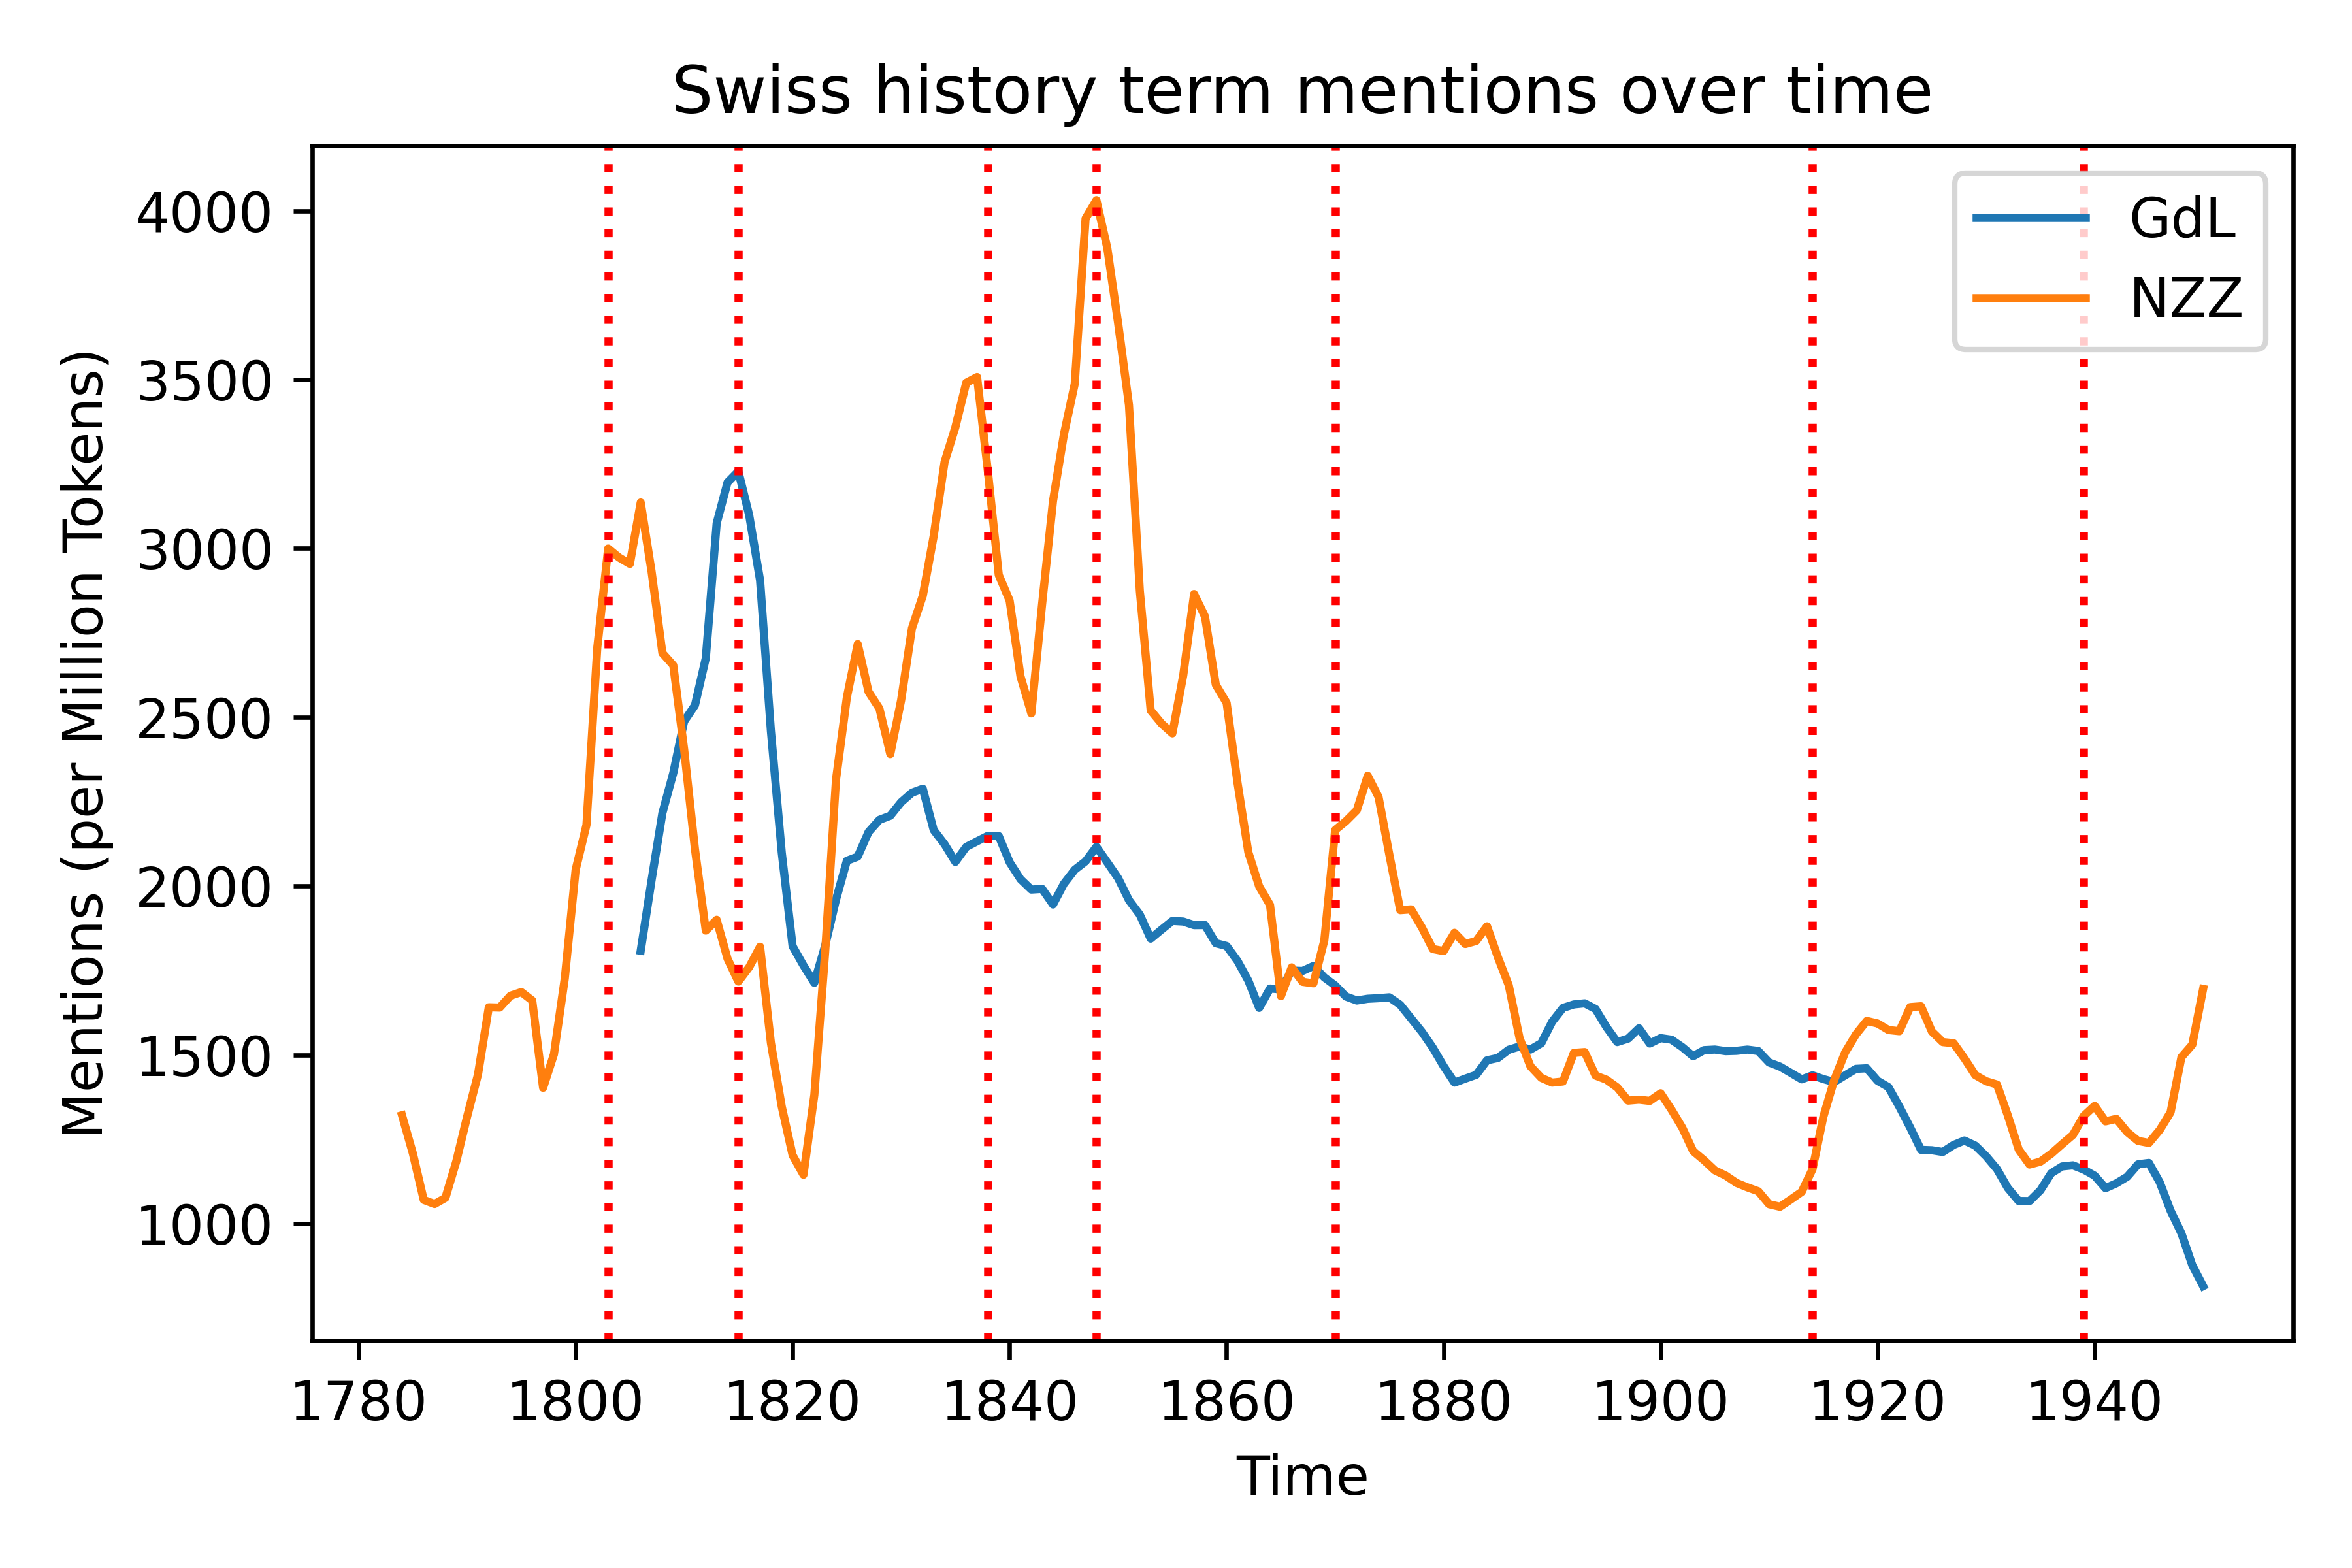
\includegraphics[width=1\linewidth]{figures/History_swiss_identity.png}
    \caption{Longitudinal analysis of cumulative frequencies of the 50 most important TF-IDF tokens in the corpus. The red lines represent important historical events:
Mediation under Napoleon (1803), Congress of Vienna (1815), Diplomatic conflict between Swiss confederacy and France (1838), Creation of modern Switzerland (1848), Creation of Italy and Germany (1870), Beginning of I. World War (1915), Beginning of II. World War (1939).
}
    \label{fig:cumulative_history}
\end{figure}




\subsection{Political Sociology}
The n-grams extracted from the political sociology sources are reported in Appendix 5. The extraction, mirroring the focus of the sources, shapes a concept of national identity based on the role of community, state politics, and of construction (or invention) of shared values\footnote{Some words that are particularly representative of this vision are 'convention', 'droit', 'etat',  'politique', 'patrie', 'culture', 'tradition', 'peuple', 'inventer', 'sentiment',  'politisch', 'staat', 'geschichte', 'politische', 'reich', 'einheit', ..}. In particular, the terms extracted delineate a concept of nation that is biased towards a cultural representation, where the nation is voluntary (the already mentioned concept of Willensnation). \par
The words for the French and the German extraction appear radically different. This diversity is motivated by the sources, as words are likely to encode aspects inherent to the two countries of Germany and France, other than only Switzerland. Accordingly, the words can be interpreted in terms of how the two sets can be used to create a partial interpretation of the Swiss nation as seen under the influence of neighboring countries. In this sense, we analyze the resulting words in terms of how, and to what extent, the conveyed socio-political representation of the national identity of the two neighboring nations can be used to model the share of Swiss identity that is a projection of its neighbors. \par
Looking at the expressions extracted from the French corpus, the representation of nation appears rather abstract \footnote{sens, sentiment, identité, definition, volunté}. The concept is tightly linked to words referring to a patriotic feeling\footnote{patrie, patriotisme, patriote}, which is a distinctive aspect of French Nationalism and the French Revolution. Patriotism is also significant in the Swiss case, which witnessed a rise of patriotism around the 1760s and a boom during the French Revolution (\citep{zimmer1999forging}). Swiss patriotism was funded upon the invocation of a glorious past and veneration of the Swiss Confederation during the 14th and 15th centuries. Among the French words, a large deal of importance is given to the n-grams representing nationalist thinkers and theories. Among these, the aforementioned 'imagined community' by Anderson figures in the top 50 list, and an ever greater resonance can be seen in the bigram 'invented traditions'. The expression was coined by Hobsbawm, and it indicates the action of the nationalist elites who shape and construct how a nation enters the public discourse (\citep{anderson2006imagined, hobsbawm2012invention}). In this view, public rituals, ceremonies, and national symbols are nothing more than utilitarian inventions of those striving to create the nation. In line with the patriotic nature of Swiss nationalism, this view mirrors the great effort of creation of Swiss identity employing myths and symbols, which culminated in the ceremonies of celebration of the Swiss nation of 1891 and 1937 (\citep{zimmer1999forging, wimmer2011swiss}). \par
Regarding the German words, attention is given, contrarily, to both abstract aspects and physical ones. We see the appearance of temporal terms\footnote{19 jahrhundert, hälfte 19, französische revolution, 20 jahrhundert}, indicating a greater focus on the temporal evolution of the concept in the German corpus, but also terms referring to cultural and sportive activities such as singers and gymnast movement\footnote{sängerbewegung and turnbewegung}. As it becomes evident by the excessive use during the Nazi and Fascist regimes, attention to sportive activities is a profound source of national sentiment, rooted in the political aesthetics of the performance \citep{rossol2010performing}. Many terms, moreover, refer to the military\footnote{militärisch, krieg, stark}, yet another symbol of national power and pride. Both sportive activities and military are elements at the root of Swiss identity, as epitomized by the Olympics and the pride put into the military system \citep{seippel1900schweiz}. The German words acquire a somewhat socialist and constructivist connotation, stressing the importance of the Volk and the social sphere, positing attention to Nationsbildung (nation-building), which morphologically implies a concept of nation that has to be constructed by the population. \par
Altogether, the two words extractions define the Swiss nation as a Willensnation based on common ideals and values and regulations. The most frequent regulations that appear are nationality law\footnote{nationalitè droit, distinguishing citizenship from statelessness}, and naturalization\footnote{naturalisation}. This latter, morphologically based on the Latin natura (nature, natural state) is, counter-intuitively, the acquisition of the nationality and the formal entrance in the social state. In the Swiss nation, naturalization is based on normative elements as well as on values\footnote{'The applicant must be well integrated, The applicant must be familiar with life in Switzerland, The applicant must not endanger Switzerland's interior or exterior security, The applicant must show respect for public order and security, The applicant must respect the values of the federal constitution, The applicant must be able to communicate in a national language, both orally and in writing, The applicant must participate in the economy or be in education, The applicant must, if married, in a registered partnership, or a parent, encourage and support the integration of his or her spouse and/or minor children' from Wikipedia on Naturalisation}. This term is one of the driving words in the longitudinal plot in \ref{fig:cumulative_sociology}, peaking in frequency in 1848 (see Appendix 7). It often resonates with articles citing or explaining the constitution (as can be seen again in Appendix 7), which explains the peak in attention in 1848, the year of publication of the Swiss constitution. 

In the aggregated trend in Figure \ref{fig:cumulative_sociology}, high resonance is achieved around 1848 and coinciding with the official creation of the nation. However, higher frequencies are found for the French part right before the Diplomatic conflict between the Swiss and French (in 1838) and the completion of the nationalist movements in Italy and Germany. Therefore, the trend seems to be anticipating international events, indicating a public discourse about nationalism in the French-speaking part in conjunction with conflicts in/with the neighboring countries. On the other hand, the trend for the German is instead reaching maximum resonance during the World Wars, where, as expected, the military and cultural symbols of the nation, which were predominantly extracted in the German words, were mentioned frequently to invoke a Swiss spirit during the wars. 


\begin{figure}[H]
    \centering
    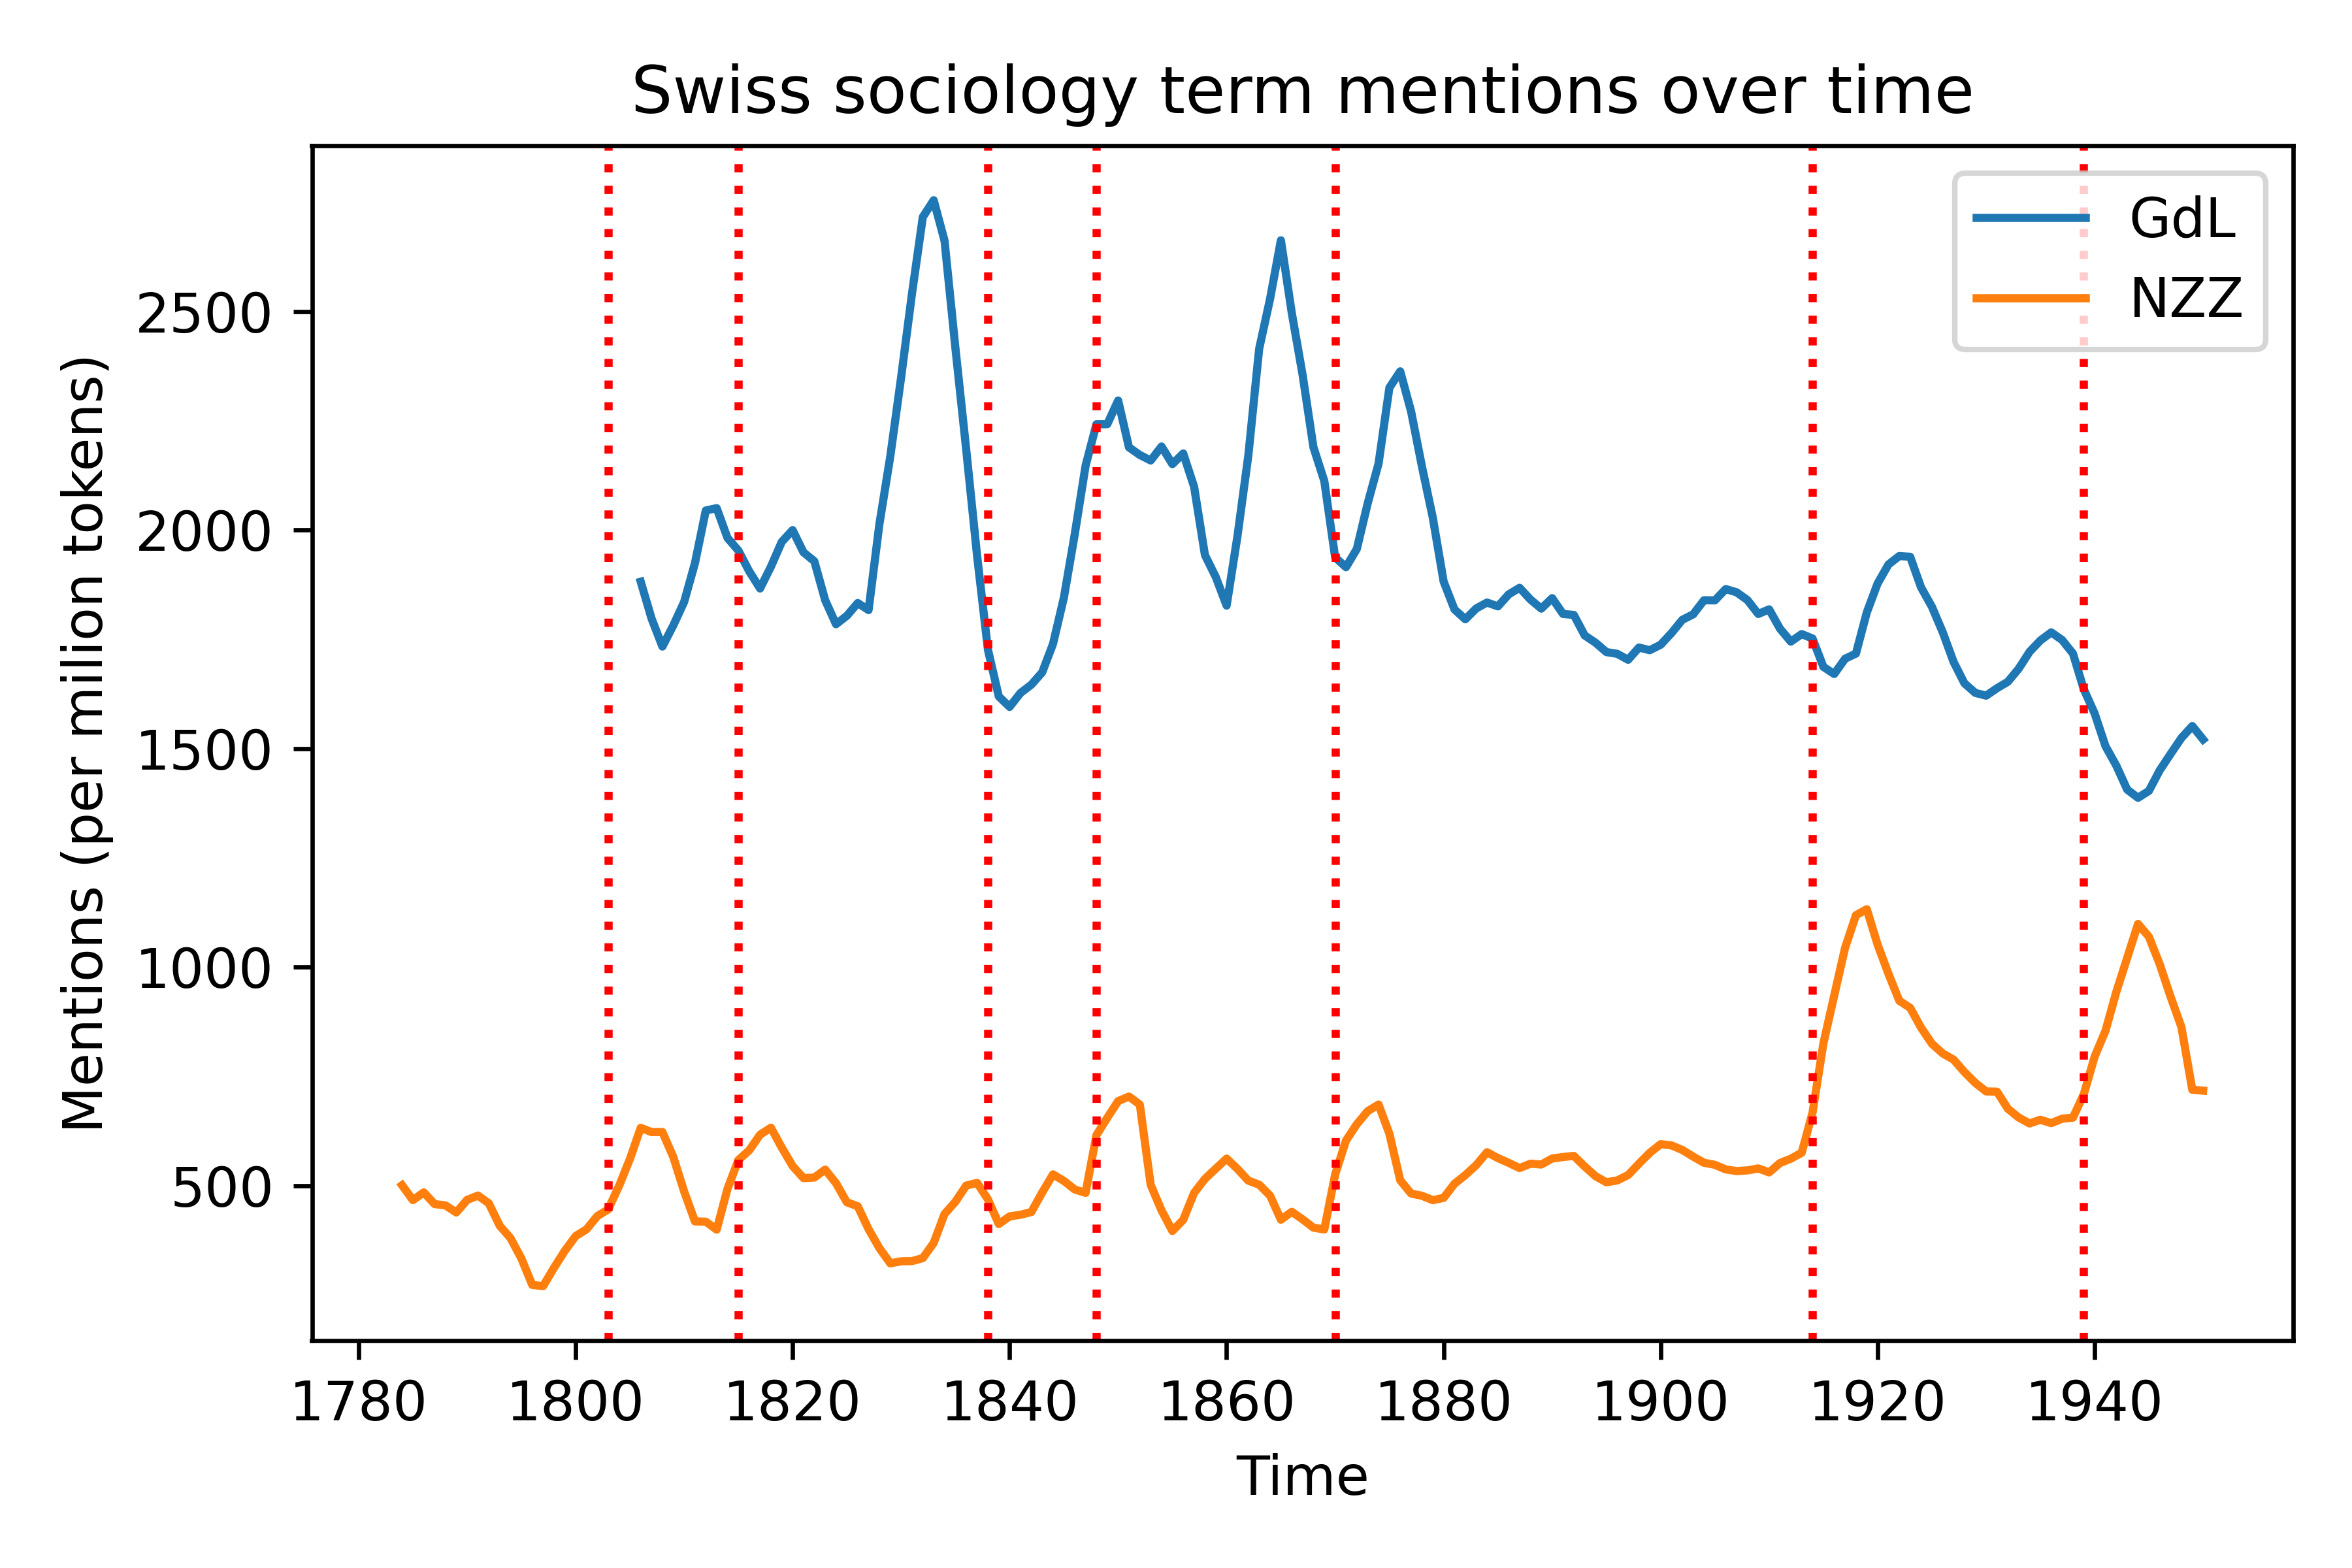
\includegraphics[width=1\linewidth]{figures/mentions_sociology.png}
    \caption{Longitudinal analysis of cumulative frequencies of the 50 most popular TF-IDF tokens in the corpus. The frequencies are normalized per million tokens. The red lines represent the following important dates: Mediation under Napoleon (1803), Congress of Vienna (1815), Diplomatic conflict between Swiss confederacy and France (1838), Creation of modern Switzerland (1848), Creation of Italy and Germany (1870), Beginning of I. World War (1915), Beginning of II. World War (1939).}
    \label{fig:cumulative_sociology}
\end{figure}


\subsection{WWI Propaganda}
Considering that we used war vs. non-war years newspapers for the WWI propaganda extraction, it is reasonable that all the factual information about the war will be present as the important tokens. Therefore, we did not take into account any terms which explicitly refer to the military. The remaining terms were closely analyzed in terms of their possible propaganda use. Finally, we decided to elaborate on three topics, which were frequent in the TF-IDF scores and essential in Swiss internal affairs during the wars. \par
The Red cross (tokens: croix rouge) is an organization of great importance for the perception of the Swiss during the war conflicts, both in foreign and internal relations. Its position and recognition were sizably increased during the first World War. Internally, the actions taken by the red cross could have been perceived as Swiss participation in the conflict, but not as an armed force but as a humanitarian power. It might have been essential for the population to criticize the government for not taking any action during the major conflict. For external politics, the actions taken by the red cross boosted the perception of Switzerland as a neutral country. \par

Swiss Neutrality (tokens: pays neutre, neutral staat, neutral land) is an important concept, which was the key point of the Swiss political coherence during the major conflicts.The narration of opposition, the Swiss unlikeness, which allowed them to stay neutral (\emph{neutral staat}) while the continent was in the tragic conflict (\emph{kriegführend staat}), was a tightly integrating collaborative sentiment. 

Swiss Railways took an important role in country integration, considering the challenging travel conditions and the prior alienation of small mountain villages. The project, which was a great achievement both in infrastructure and nation-building, mainly took part in the XIX and the beginning of the XX century. It paved the way for fast information and ideas sharing through the country and made a Swiss internal integration a much more convincing alternative to cross-border integration, which could otherwise take place for each part of Switzerland independently, decreasing the national coherence. \par

\begin{figure}[H]
    \centering
    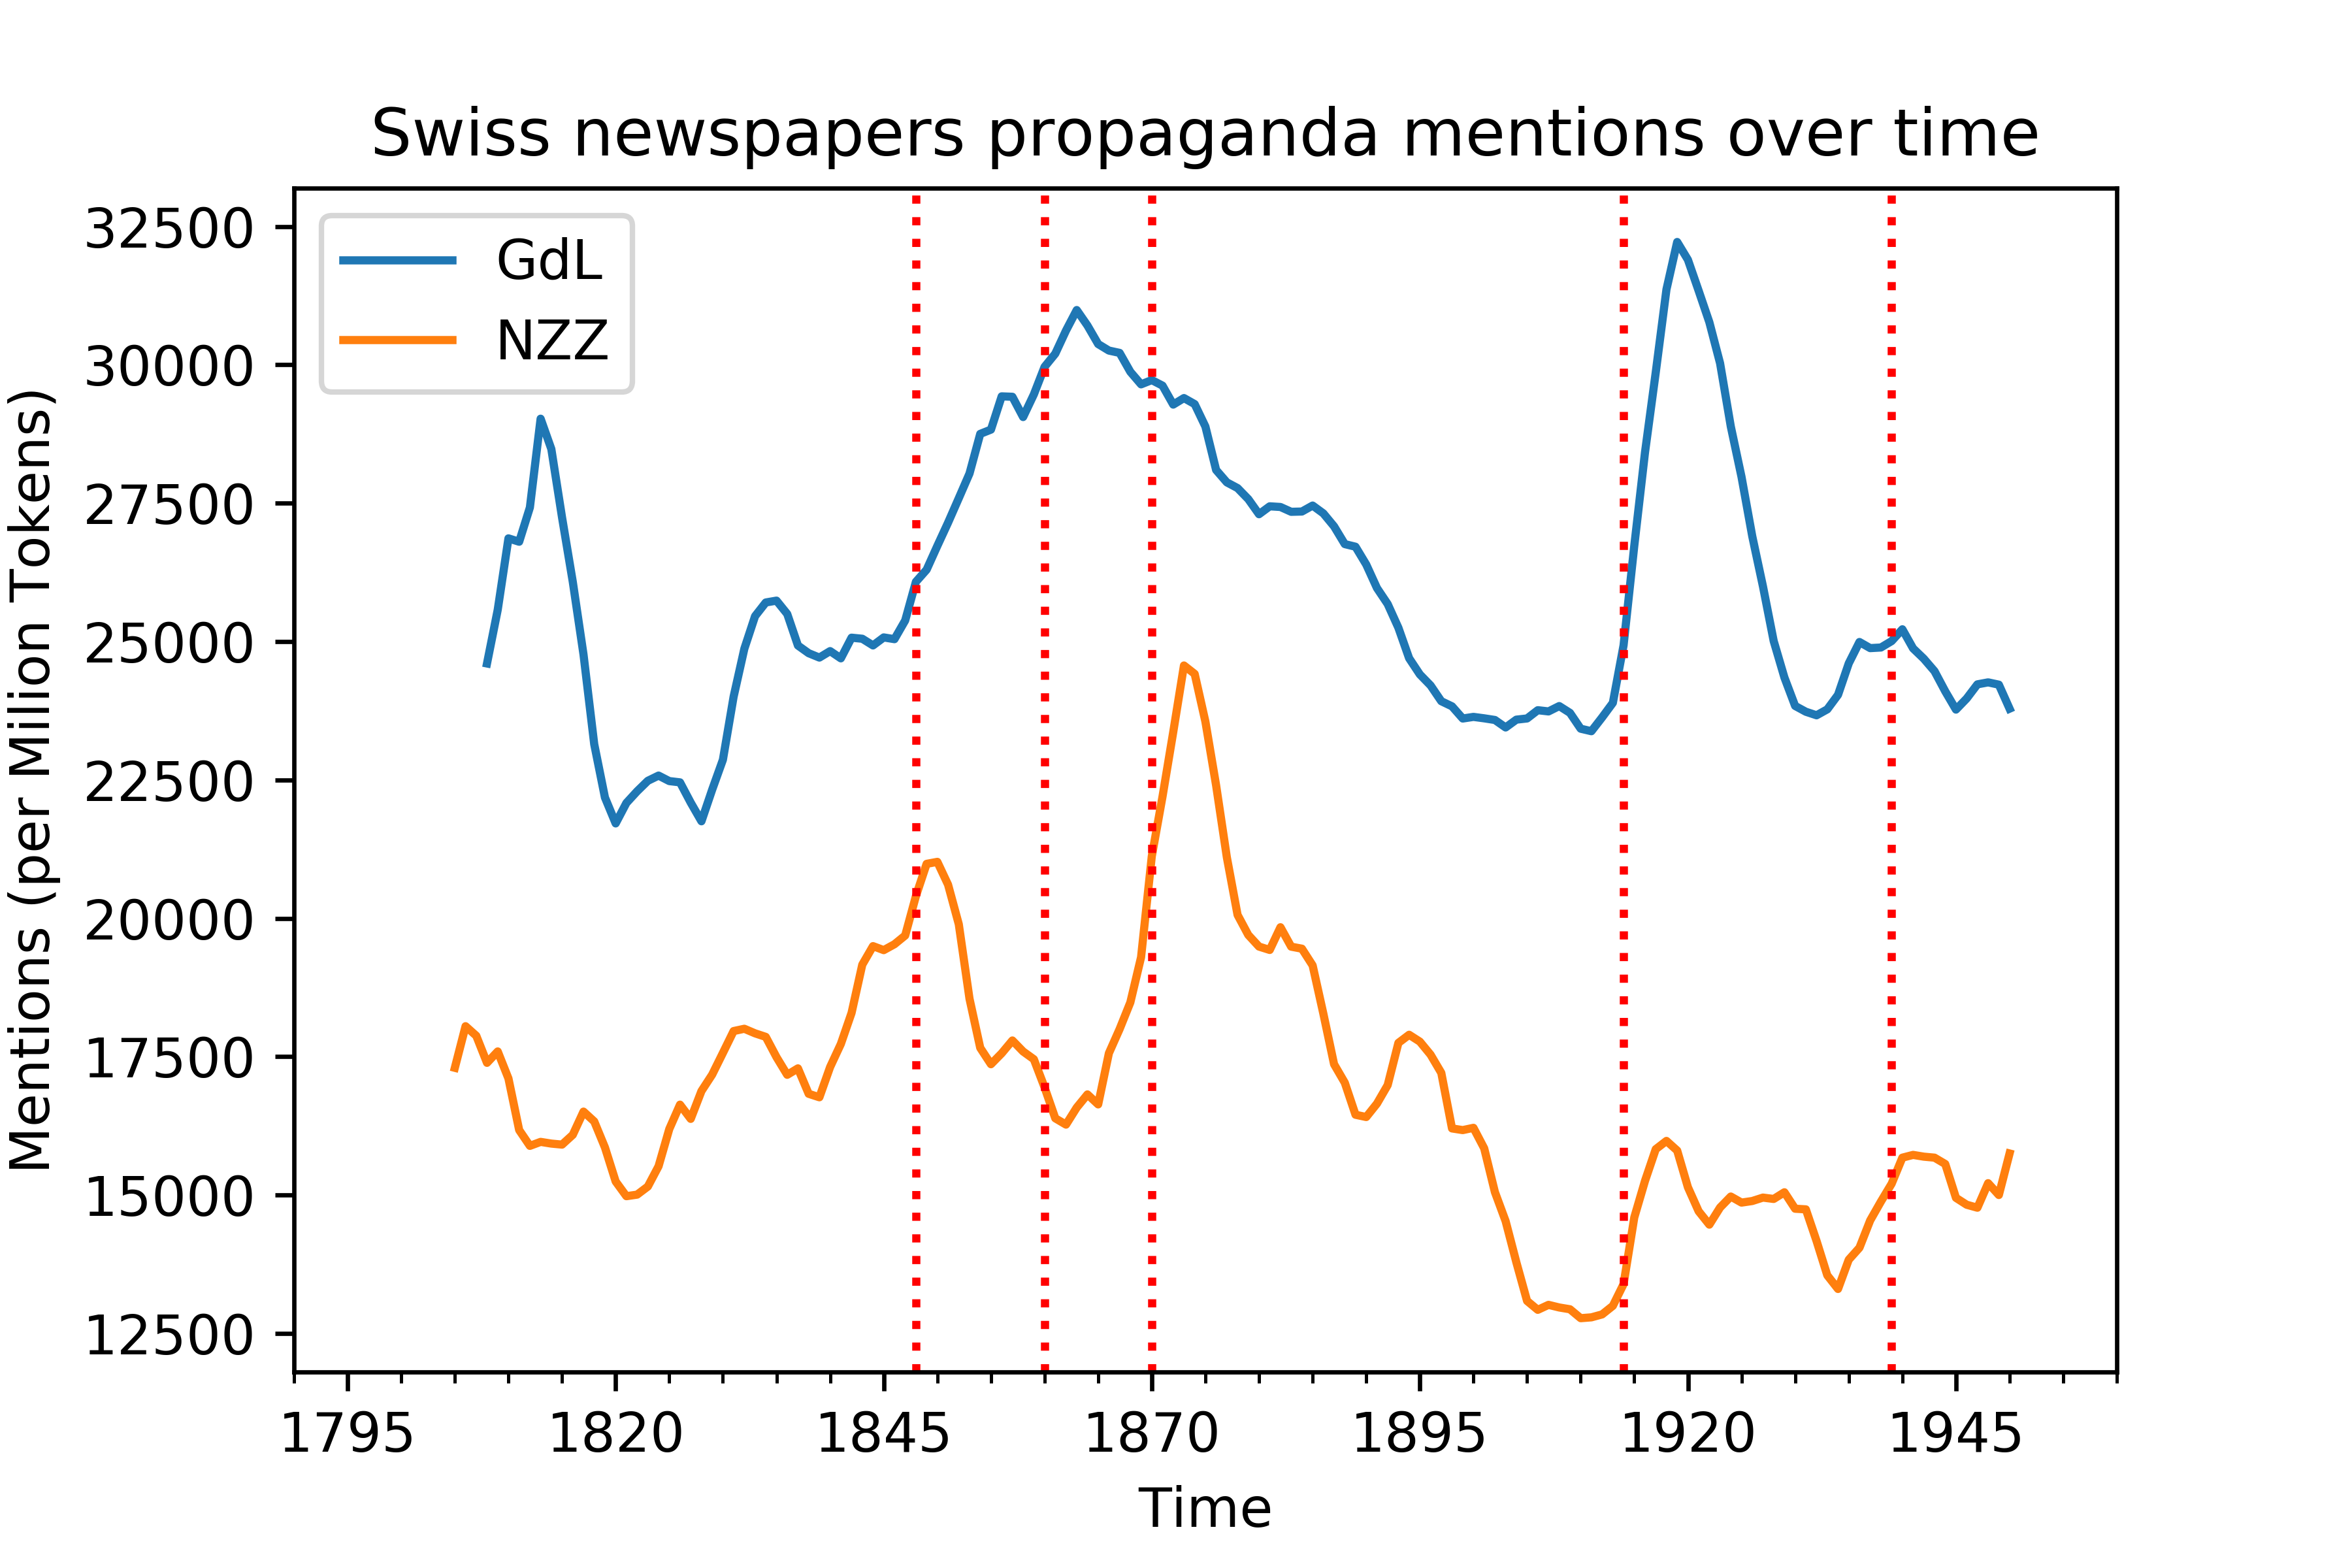
\includegraphics[width=1\linewidth]{figures_Michal/cumulative_propaganda.png}
    \caption{Longitudinal analysis of cumulative frequences of the most popular TF-IDF tokens in the corpus. The red lines represent important conflicts: Sonderbunden war, Savoy conflict, Franco-Prussian war, WWI, WWII}
    \label{fig:cumulative_propaganda}
\end{figure}

The detailed trend visible in Figure~\ref{fig:cumulative_propaganda}, alongside the full TF-IDF result tables, available in Appendix 6, provides some interesting insights into the Swiss newspapers' propaganda. First, there is a visible trend of propaganda increase, consistent with the appearance of political situations dangerous for Swiss integrity. Secondly, while the Franco-Prussian war and WWI remain of the highest importance, the other situations seem to be covered more locally only in the more active part of Switzerland. Finally, we note nearly complete Swiss indifference to WWII, which is surprising but might be explained by the success of the WWI armed neutrality strategy and the broad consensus of Swiss public opinion that the same strategy might work again.


\newpage

\section{Discussion \& Conclusions}
The extraction methods presented, the resulting sets of words depicting national identity, and the final aggregated trends create a considerable overhead in the results. Therefore, a conclusion is crucial and critical, and similarities and differences in the produced results need to be explained.\par
First, considering the resulting terms, different concepts and topics describing Swiss national identity have been detected within each obtained term list. Terms that encode locations or important historical protagonists constitute one of the common topics to all extractions. This topic, however, is somewhat unsurprising, thus discarded by this paper. A topic of interest is that which places Switzerland in relation with the international, relating Switzerland and neighboring European powers. This topic is present in all three sources, although the precise functionality varies across the sources. In the historical sources, the surrounding powers seem to be the acting powers that force the Swiss cantons to build an alliance, which eventually would yield into a nation. The WWI propaganda shows a cemented nation resisting external forces. Lastly, the sociological papers depict Switzerland as influenced by its surrounding countries. The substantial focus on external powers to define Swiss sentiment in all three sources indicates that the definition of Swiss nationhood is bound to discriminate between Swiss and non-Swiss.  \par
Moreover, the topic of Switzerland's neutrality and its military recur in all extractions. Its connotation varies again between the sources; however, parallels in its functionality can be found across all sources. First, the historical sources reflect the importance of the Swiss military alliance and its resistance against outside powers. This narrative is continued by the WWI propaganda, which also strongly focuses on Swiss neutrality. At last, the sociological papers reflect on the cohesive powers of the shared military service and shared experience of resistance as symbols for constructing the identity.\par
A last, rather abstract topic, mainly covered by historical and political sources, describes political participation and institutions. Here the obtained terms seem to draw on two opposing concepts. One indicates that Swiss national identity is an invention of local elites and the other that the Swiss nation is deeply rooted in the population by a sort of collective awareness and memory. This dichotomy reflects the discourse of Switzerland as both a voluntary nation (Willensnation) or a natural community (Wesensgemeinschaft) \citep{zimmer1999forging} introduced in the Research Context.\par

The time trends obtained by each term list partially mirror each other but vary in magnitude and accentuation. It is visible that each source is a biased representation of its own time and thus yields higher trends during its respective time frame. However, the obtained time trends draw peaks in term mentions which coincide with significant historical events. Those historical events are either internal or external conflicts, which question or redefine the Swiss nation. During such events, the investigated newspapers use a vocabulary that reflects or predetermines the terms that were computationally obtained. 
The usage of national identity-defining words during internal or external conflict and restructuring might indicate that Swiss national identity still had to be solidified over the XIX century. However, it seems that the peak indicating the beginning of the Second World is lower and less significant in all three plots. The decrease in importance might signify that during WWII, Swiss nationalism was solidified to the point that less public discussion was necessary to convey Swiss national identity.

The overall picture of Swiss identity traced by this project can be summarized as follows: It is a process that is boosted by internal or external conflicts, by the need to define the Swiss from the non-Swiss. It is also a concept shaped by both political and cultural factors, by abstract and concrete ones. It relies on the symbols of military honors and sports ceremonies. It also relies on a shared past rich of ideals of democracy, neutrality, and driven by a strong patriotism.

However, this reconstruction is inherently limited, and it is important to acknowledge its limitations. Firstly, the term extraction is mainly biased in two directions: temporally and thematically. It is plausible that each source type resonates most with the language and events of the time the source was made; hence, there is an increase in frequency around the time of the sources. Furthermore, each source depicts only a partial view of the nation, the first based on political-historical events, the second on demagogic myths and values, and the last on abstract definitions of nationality. The already biased and lateral view of the Swiss nation is further problematized by the inherent limitations of the TF-IDF method, which can determine which words are rather specific to a document but cannot distinguish which words are more valuable than others. More specifically, the algorithm has no concept of the semantics of the words; thus, it cannot filter out infrequent words with very general meanings or words that distance too much from the concept of nation. This limitation also introduces the need for vast manual filtering when analyzing the extracted words. \par
Moving to the frequency-time trends, properly normalizing the frequencies in time and across newspapers is complex. Although currently, this paper normalizes by million tokens (so how many times a word appears every million tokens published in the newspaper in the specific year), this does not take into account the actual total number of articles in the year, nor in the Swiss region nor among a newspaper's specific edition. It does not indicate how relevant a word is to the unit of the article, and it weighs too heavily when a word appears several times in the same article. Moreover, when a peak is detected, it is not easy to separate when the mention is about the Swiss case or an international event. It is also challenging to understand whether the word extracted was used in the article with the same connotation it had when it was extracted. For instance, the 'XIX century' can be mentioned about the rise of nationalism but also in various other contexts. Finally, the language barrier between the French and German corpora extractions makes the comparison between the two languages and corresponding trends almost impossible. \par

Extensive future work is needed to overcome these limitations. A first step, which was partly tried in Appendix 7, is to investigate the context in which the words were used in the newspapers to check that they are used with the intended meaning and better understand the modalities with which Swiss identity was treated. Another step consists of extracting more similar words for the two languages, addressing the translation between one and the other, either by using the same corpora for the extraction or just translating the extracted words. Expansions to obviate the problems inherent to the method are to expand the reference corpora to texts treating nationalism of other countries (but not Switzerland, to extract more 'Swiss nationality' terms), and filter words using word embeddings and a distance measure from the concept of nationality. We also acknowledge that a complete analysis of the Swiss identity should also extend to Romansh and Italian sources.\par
Despite these limitations, this project, aided by vast research and manual analysis, could produce numerous and convincing results describing Swiss national identity. Most importantly this includes the quantitative representation of the account of Swiss national identity which was delineated by the given sources and its numerical evolution over time.


\newpage

\bibliographystyle{apalike}
\bibliography{references}

\newpage
\pagestyle{empty}
\section*{Appendix 1: Sociology Corpus}
Following is the list of papers used for expression extraction from a political sociology side:\\

\noindent\textbf{French:}

\begin{enumerate}
    \item Ipperciel, D. (2001). \textit{Habermas, Taylor et le nationalisme québécois. }Dialogue: Canadian Philosophical Review/Revue canadienne de philosophie, 40(3), 529-544.
    \item Babadzan, A. (1999). \textit{L'invention des traditions et le nationalisme}. Journal de la Société des Océanistes, 109(2), 13-35.
    \item Ipperciel, D. (2007). \textit{La Suisse: un cas d'exception pour le nationalisme?}. Swiss political science review, 13(1), 39-67. Godechot, J. (1971, October). \textit{Nation, patrie, nationalisme et patriotisme en France au XVIII e siècle}. In Annales historiques de la Révolution française (pp. 481-501). Soci t des Etudes Robespierristes.
    \item Gellner, E. (1991).\textit{ Le nationalisme en apesanteur}. Terrain. Anthropologie et sciences humaines, (17), 7-16.
    \item Hermet, G. (1997).\textit{ Populisme et nationalisme.} Vingtième siècle. Revue d'histoire, 34-47.
    \item Dieckhoff, A. (1996). \textit{La déconstruction d'une illusion. L'introuvable opposition entre nationalisme politique et nationalisme culturel}. L'Année sociologique (1940/1948-), 43-55.
    \item Gutzwiller, C. (2008). \textit{Droit de la nationalité et fédéralisme en Suisse}. Schulthess.
    \item Darmau, F. (1988). \textit{Les ambiguïtés de Renan: Nation, Nationalisme, Internationalisme.} Raison présente, 86(1), 27-35.
    \item Argast, R. and Arlettaz, S. and Arlettaz, G. (2003). \textit{Citoyenneté, nationalité et formation nationale en Suisse 1798-1925.} In Sonderdruck aus: Studien und Quellen/Etudes et Sources-Integration und Ausschluss/Intégration et Exclusion (No. 29, pp. 129-160). Haupt.
    \item Lalande Bernatchez, J. (2013). \textit{Aux limites de la nation: les théories du nationalisme et le débat conceptuel sur l'articulation du racisme et du nationalisme}.
    \item Laszlo Ledermann (1959). \textit{La Nationalisme et sa Signification pour les Relations Internationales.} Contribution à une étude historique et psycho-sociale. (E-Periodica)
\end{enumerate}

[3,8,10] are specifically about the Swiss case, [1,9] are commentaries of other authors, and [12] is an E-Periodica article (not a peer reviewed paper).\\

\noindent\textbf{German: }

\begin{enumerate}
    \item Scriba, F. (2007). \textit{Siegfried Weichlein, Nationalbewegungen und Nationalismus in Europa, Darmstadt}. Comparativ, 17(1), 141-143.
    \item (2000). \textit{Dossier : die Schweiz - eine Utopie?} Zeitschrift: Schweizer Monatshefte : Zeitschrift für Politik, Wirtschaft, Kultur. (E-Periodica)
    \item Imhof, K. (1993). \textit{Nationalismus, Nationalstaat und Minderheiten: Zu einer Soziologie der Minoritäten}. Soziale Welt, 327-357.
    \item Langewiesche, D. (2000). \textit{Nation, Nationalismus, Nationalstaat in Deutschland und Europa} (Vol. 1399, p. 267). Beck.
\end{enumerate}

[2] is an E-Periodica dossier about the Swiss case.

\section*{Appendix 4: TF-IDF results for Swiss history corpus}
\label{appendix4}

\begin{table}[H]
\begin{center}
\begin{small}
\captionof{table}{\small Top 50 French n-grams from Swiss history books ordered by TFIDF values}
\label{TFIDF_Terms_Top_Twenty_hist_Fr}
\begin{tabular*}{\textwidth}{|l|| @{\extracolsep{\fill}} l c || l c |} 
\hline
Rank & Unigram & TFIDF Value  & Bigram & TFIDF Value \\
\hline
\hline
0   &     rodolphe  &  0.332393  &            comte pierre  &  0.094145  \\
1   &        comte  &  0.245470  &          comte rodolphe  &  0.081070  \\
2   &      tschudi  &  0.221161  &            comte savoie  &  0.071235  \\
3   &        berne  &  0.198825  &         abbé saint-gall  &  0.054139  \\
4   &        ville  &  0.158460  &             ville berne  &  0.054139  \\
5   &       zurich  &  0.147189  &        maison habsbourg  &  0.051289  \\
6   &       albert  &  0.119029  &             marc argent  &  0.048720  \\
7   &           ch  &  0.117110  &      rodolphe habsbourg  &  0.048440  \\
8   &       suisse  &  0.116733  &           comte palatin  &  0.047073  \\
9   &    bourgeois  &  0.115486  &         bourgeois berne  &  0.042741  \\
10  &     seigneur  &  0.114379  &          comte eberhard  &  0.042741  \\
11  &          roi  &  0.107953  &          rodolphe broun  &  0.039892  \\
12  &    habsbourg  &  0.107745  &          avoyer conseil  &  0.039892  \\
13  &         jean  &  0.107196  &          jean bubenberg  &  0.039892  \\
14  &         pays  &  0.106166  &          empereur louis  &  0.039227  \\
15  &      château  &  0.105915  &          empereur henri  &  0.039227  \\
16  &       charte  &  0.102741  &            comte amédée  &  0.037042  \\
17  &       évêque  &  0.102735  &         comte habsbourg  &  0.037042  \\
18  &  waldstetten  &  0.102074  &          comte hartmann  &  0.034193  \\
19  &      kibourg  &  0.093001  &           comte kibourg  &  0.034193  \\
20  &       guerre  &  0.087685  &               cent marc  &  0.034193  \\
21  &     hartmann  &  0.087330  &         suisse allemand  &  0.034193  \\
22  &      bernois  &  0.086396  &          pierre gruyère  &  0.034193  \\
23  &       maison  &  0.083701  &     gouverneur impérial  &  0.034193  \\
24  &       schwyz  &  0.081660  &         bourgeois ville  &  0.033997  \\
25  &         abbé  &  0.077291  &       empereur frédéric  &  0.031382  \\
26  &     empereur  &  0.076203  &        bourgeois zurich  &  0.031344  \\
27  &        saint  &  0.075517  &        évêque constance  &  0.031344  \\
28  &       savoie  &  0.075300  &        maison neuchâtel  &  0.031344  \\
29  &        henri  &  0.074452  &              cent homme  &  0.028767  \\
30  &    chevalier  &  0.072443  &          rodolphe comte  &  0.028494  \\
31  &        grand  &  0.071780  &            évêque henri  &  0.028494  \\
32  &    neuchâtel  &  0.070782  &  habsbourg lauffenbourg  &  0.028494  \\
33  &          duc  &  0.070215  &             pays schwyz  &  0.028494  \\
34  &     fribourg  &  0.068758  &        comte tokenbourg  &  0.028494  \\
35  &         gall  &  0.068335  &      rodolphe neuchâtel  &  0.028494  \\
36  &     eberhard  &  0.063513  &            grand église  &  0.026151  \\
37  &         bâle  &  0.063496  &          bannière ville  &  0.025645  \\
38  &        chron  &  0.062385  &          vallée urseren  &  0.025645  \\
39  &       pierre  &  0.062333  &           louis bavière  &  0.025645  \\
40  &     alliance  &  0.062278  &              acte achat  &  0.025645  \\
41  &      couvent  &  0.061644  &           public domain  &  0.025645  \\
42  &        baron  &  0.061043  &        électeur mayence  &  0.025645  \\
43  &        temps  &  0.060852  &           rodolphe fils  &  0.025645  \\
44  &         fils  &  0.060265  &             traité paix  &  0.024361  \\
45  &        homme  &  0.060136  &            grand nombre  &  0.024163  \\
46  &        frère  &  0.058822  &              avoir lieu  &  0.023765  \\
47  &      zuricoi  &  0.057842  &          guillaume tell  &  0.023536  \\
48  &       erlach  &  0.056708  &              comte jean  &  0.023536  \\
49  &     impérial  &  0.056401  &              long temps  &  0.023479  \\
\hline
\end{tabular*}
\end{small}
\end{center}
\end{table}

\begin{table}[H]
\begin{small}
\begin{center}
\captionof{table}{\small Top 50 German n-grams from Swiss history books ordered by TFIDF values}\label{TFIDF_Terms_Top_Twenty_2}
\begin{tabular*}{\textwidth}{|l|| @{\extracolsep{\fill}} l c || l c |} 
\hline
Rank & Unigram & TFIDF Value  & Bigram & TFIDF Value \\
\hline
\hline
0 	& 	kanton 	& 	0.517982 	& 	numa droz 	& 	0.113806 	\\
1 	& 	schweiz 	& 	0.314341 	& 	französisch truppe 	& 	0.096147 	\\
2 	& 	regierung 	& 	0.165484 	& 	helvetische regierung 	& 	0.090260 	\\
3 	& 	truppe 	& 	0.153276 	& 	helvetischen republik 	& 	0.074563 	\\
4 	& 	französisch 	& 	0.146008 	& 	droz wiedergeburt 	& 	0.068676 	\\
5 	& 	zürich 	& 	0.143091 	& 	öffentlich meinung 	& 	0.066714 	\\
6 	& 	tagsatzung 	& 	0.127124 	& 	droz protektorat 	& 	0.064752 	\\
7 	& 	partei 	& 	0.126443 	& 	bull lois 	& 	0.062790 	\\
8 	& 	frankreich 	& 	0.107725 	& 	helvetische republik 	& 	0.056903 	\\
9 	& 	eidgenössisch 	& 	0.106244 	& 	helvetischen regierung 	& 	0.056903 	\\
10 	& 	helvetischen 	& 	0.095005 	& 	französisch regierung 	& 	0.049054 	\\
11 	& 	behörde 	& 	0.093347 	& 	regie rung 	& 	0.045130 	\\
12 	& 	luzern 	& 	0.090891 	& 	kanton bern 	& 	0.043168 	\\
13 	& 	droz 	& 	0.089048 	& 	ordnung ding 	& 	0.039652 	\\
14 	& 	eidgenossenschaft 	& 	0.083982 	& 	französische regierung 	& 	0.039244 	\\
15 	& 	verfassung 	& 	0.081092 	& 	vollz nathes 	& 	0.039244 	\\
16 	& 	bern 	& 	0.080510 	& 	zürich bern 	& 	0.037281 	\\
17 	& 	waadt 	& 	0.076152 	& 	prot vollz 	& 	0.037281 	\\
18 	& 	helvetische 	& 	0.075527 	& 	kanton waadt 	& 	0.037281 	\\
19 	& 	bürger 	& 	0.071599 	& 	demokratisch kanton 	& 	0.035319 	\\
20 	& 	schweizerisch 	& 	0.071504 	& 	protof vollz 	& 	0.035319 	\\
21 	& 	öffentlich 	& 	0.071504 	& 	numa droz wiedergeburt 	& 	0.035319 	\\
22 	& 	verninac 	& 	0.069396 	& 	verfassung geben 	& 	0.035319 	\\
23 	& 	erklären 	& 	0.069212 	& 	lluma droz 	& 	0.033357 	\\
24 	& 	französische 	& 	0.067636 	& 	numa droz protektorat 	& 	0.033357 	\\
25 	& 	consul 	& 	0.063209 	& 	helvetischen truppe 	& 	0.033357 	\\
26 	& 	wallis 	& 	0.063135 	& 	general bachmann 	& 	0.031395 	\\
27 	& 	juli 	& 	0.062052 	& 	heutige staatsrecht 	& 	0.031395 	\\
28 	& 	märz 	& 	0.059643 	& 	eidgenössisch truppe 	& 	0.029433 	\\
29 	& 	schwyz 	& 	0.059570 	& 	provisorische regierung 	& 	0.029433 	\\
30 	& 	republik 	& 	0.059005 	& 	helvetischen behörde 	& 	0.029433 	\\
31 	& 	bundesrat 	& 	0.058342 	& 	schwyz unterwalden 	& 	0.029433 	\\
32 	& 	freiburg 	& 	0.058055 	& 	vollz rathes 	& 	0.029433 	\\
33 	& 	helvetien 	& 	0.056364 	& 	kanton luzern 	& 	0.027470 	\\
34 	& 	volk 	& 	0.054565 	& 	vollz nath 	& 	0.027470 	\\
35 	& 	genf 	& 	0.054350 	& 	regierung bern 	& 	0.027470 	\\
36 	& 	neutralität 	& 	0.054109 	& 	kanton zürich 	& 	0.027470 	\\
37 	& 	mehrheit 	& 	0.053847 	& 	schweiz frankreich 	& 	0.025508 	\\
38 	& 	abgeordnete 	& 	0.053783 	& 	wirtschaftlich schwierigkeit 	& 	0.025508 	\\
39 	& 	basel 	& 	0.053031 	& 	solothurn basel 	& 	0.025508 	\\
40 	& 	militärisch 	& 	0.052815 	& 	basel schaffhausen 	& 	0.023546 	\\
41 	& 	minister 	& 	0.052291 	& 	bern luzern 	& 	0.023546 	\\
42 	& 	rat 	& 	0.051857 	& 	französisch gesandte 	& 	0.023546 	\\
43 	& 	reding 	& 	0.051587 	& 	einzeln kanton 	& 	0.023546 	\\
44 	& 	politisch 	& 	0.051028 	& 	bull hely 	& 	0.023546 	\\
45 	& 	dezember 	& 	0.050972 	& 	neutralität schweiz 	& 	0.023546 	\\
46 	& 	land 	& 	0.050874 	& 	achtzehnten jahrhundert 	& 	0.023546 	\\
47 	& 	aargau 	& 	0.050164 	& 	aufrecht erhalten 	& 	0.021820 	\\
48 	& 	juni 	& 	0.050142 	& 	kantonalen revolution 	& 	0.021584 	\\
49 	& 	bonaparte 	& 	0.049744 	& 	kanton aargau 	& 	0.021584 	\\
\hline
\end{tabular*}
\end{center}
\end{small}
\end{table}

\newpage

\section*{Appendix 5: TF-IDF results for political sociology corpus}

\begin{table}[H]
\begin{center}
\begin{small}
\captionof{table}{\small Top 50 French n-grams from political sociology corpus ordered by TFIDF Values}
\label{TFIDF_Terms_Top_Twenty_Fr}
\begin{tabular*}{\textwidth}{|l|| @{\extracolsep{\fill}} l c || l c |} 
\hline
Rank & Unigram & TFIDF Value  & Bigram & TFIDF Value \\
\hline
\hline
0   &     nationalisme  &  0.53  &            racisme nationalisme  &  0.25  \\
1   &        nationalité   &  0.32  &         droit nationalité  &  0.14  \\
2   &      nation  &  0.25  &            théorie nationalisme  &  0.11  \\
3   &        racisme  &  0.23  &         convention nationalité  &  0.09  \\
4   &        suisse   &  0.19  &            théoricien nationalisme  &  0.08  \\
5   &       convention   &  0.17  &        tradition inventer  &  0.07  \\
6   &       droit   &  0.14  &             convention européen  &  0.06  \\
7   &           etat   &  0.14  &      droit homme  &  0.06  \\
8   &       national   &  0.12  &           art convention  &  0.06  \\
9   &    politique   &  0.11  &         mot patrie  &  0.06  \\
10  &     patrie   &  0.11  &          nationalisme racisme &  0.06  \\
11  &          anderson   &  0.11  &         articulation racism &  0.06  \\
12  &    smith   &  0.10  &articulation racisme nationalisme  &  0.06  \\
13  &         culture   &  0.09  &      lien racisme  &  0.05  \\
14  &         tradition   &  0.09  &         lien racisme nationalisme  &  0.05  \\
15  &      culturel   &  0.08  &         convention européen nationalité  &  0.05  \\
16  &       peuple   &  0.07  &           invention tradition  &  0.05  \\
17  &       nationaliste   &  0.06  &        européen nationalité  &  0.05  \\
18  &  hobsbawm   &  0.06  &          naturalisation ordinaire  &  0.04  \\
19  &      voir   &  0.06  &          explicatif convention européen  &  0.04  \\
20  &       naturalisation   &  0.06  &     art let  &  0.04  \\
21  &     nairn   &  0.06  &        rapport explicatif convention européen  &  0.04  \\
22  &      habermas   &  0.06  &    rapport explicatif convention  &  0.04  \\
23  &       nationaliter   &  0.06  & rapport explicatif  &  0.04  \\
24  &       social   &  0.05  &         nationalité droit  &  0.04  \\
25  &         nationalism   &  0.05  &      explicatif convention  &  0.04  \\
26  &     langue  &  0.05  &     droit international  &  0.04  \\
27  &        moderne   &  0.05  &       nationalité numéro  &  0.04  \\
28  &       europe   &  0.05  &        nation moderne &  0.04  \\
29  &        patriote   &  0.05  &          mot nation  &  0.04  \\
30  &    gellner   &  0.05  &         relation racisme  &  0.03  \\
31  &        renan   &  0.05  &   convention européen nationalité numéro  &  0.03  \\
32  &    homme   &  0.05  &  anthony smith  &  0.03  \\
33  &          mot   &  0.05  &  explicatif convention européen nationalité  &  0.03  \\
34  &     principe   &  0.05  &  droit fondamental &  0.03  \\
35  &         phénomène   &  0.05  &      européen nationalité numéro  &  0.03  \\
36  &     linguistique   &  0.04  &            espace public  &  0.03  \\
37  &         art   &  0.04  &          let convention nationalité  &  0.03  \\
38  &        question   &  0.04  &          let convention  &  0.03  \\
39  &       citoyen   &  0.04  &           benedict anderson  &  0.03  \\
40  &     pouvoir   &  0.04  &           art convention nationalité  &  0.03  \\
41  &      rapport   &  0.04  &           procédure naturalisation  &  0.03  \\
42  &        naim   &  0.04  &     art let convention nationalité  &  0.03  \\
43  &        patriotisme   &  0.04  &        batiffol henri  &  0.03  \\
44  &         public   &  0.04  &     relation racisme nationalisme &  0.03  \\
45  &        sens   &  0.04  &        art let convention  &  0.03  \\
46  &        théoricien   &  0.04  &       général droit &  0.03  \\
47  &      inventer   &  0.04  &        imagined communities  &  0.03  \\
48  &       sentiment   &  0.04  &      nationalité art  &  0.03  \\
49  &     cas   &  0.04  &          borella françois  &  0.03  \\
\hline
\end{tabular*}
\end{small}
\end{center}
\end{table}

\begin{table}[H]
\begin{center}
\begin{small}
\captionof{table}{\small Top 50 German n-grams from political sociology corpus ordered by TFIDF values}
\label{TFIDF_Terms_Top_Twenty_Ge}
\begin{tabular*}{\textwidth}{|l|| @{\extracolsep{\fill}} l c || l c |} 
\hline
Rank & Unigram & TFIDF Value  & Bigram & TFIDF Value \\
\hline
\hline
0   &     nation  &  0.46  &           deutsch nation  &  0.19  \\
1   &        nationalstaat    &  0.30  &          19 jahrhundert  &  0.19  \\
2   &      deutsch   &  0.23  &         deutsch nationalstaat  &  0.11  \\
3   &        nationalismus   &  0.23  &    deutsche bund  &  0.10  \\
4   &       national    &  0.17  &  deutsch staat  &  0.09  \\
5   &       europa    &  0.16  &     nation nationalstaat  &  0.07  \\
6   &       politisch    &  0.14  &     deutsch geschichte  &  0.07  \\
7   &       schweiz    &  0.13  &   hälfte 19 jahrhundert  &  0.06  \\
8   &       staat    &  0.13  &      modern nationalismus &  0.06  \\
9   &    österreich    &  0.12  &     hälfte 19  &  0.06  \\
10  &     revolution    &  0.12  &    schwäbisch sängerbewegung  &  0.06  \\
11  &         deutschland    &  0.10  &    deutsch nationalbewegung &  0.06  \\
12  &    jahrhundert    &  0.10  &  18 jahrhundert  &  0.05  \\
13  &        volk    &  0.09  &    prozeß nationsbildung  &  0.04  \\
14  &        nationsbildung   &  0.09  &    idee nation  &  0.04  \\
15  &     19    &  0.09  &     schwäbische sängerbewegung  &  0.04  \\
16  &   geschichte    &  0.09  &     national bewegung  &  0.04  \\
17  &   politische    &  0.08  &   modern nation  &  0.04  \\
18  &  reich    &  0.08  &        20 jahrhundert  &  0.03  \\
19  &      jahn    &  0.08  &     französische revolution &  0.03  \\
20  &       einheit   &  0.08  &        alte reich  &  0.03  \\
21  &     sängerbewegung   &  0.08 &   deutsch sängerbewegung  &  0.03  \\
22  &     entstehen    &  0.07  &     schwäbisch sängerbund  &  0.03  \\
23  &    krieg   &  0.07  &   schwäbische sängerbundes  &  0.03  \\
24  &   schwäbisch   &  0.07  &     deutsch volk  &  0.03  \\
25  &       fremde   &  0.07  &      spät 18  &  0.03  \\
26  &     frankreich   &  0.07  &     idee deutsch  &  0.03  \\
27  &       europäisch   &  0.06  & partizipation aggression  &  0.03  \\
28  &       kulturell   &  0.06  &    kleindeutschen nationalstaat  &  0.03  \\
29  &       gesellschaft   &  0.06  &   staat gesellschaft  &  0.03  \\
30  &    preuße   &  0.06  &     otto elben  &  0.03  \\
31  &       idee   &  0.06  &     19 20  &  0.03  \\
32  &    deutsche   &  0.06  & sozial bewegung  &  0.02  \\
33  &          leben    &  0.06  &      karl pfaff  &  0.02  \\
34  &     bund    &  0.06  &      frage stellen  &  0.02  \\
35  &         turnbewegung  &  0.06  &    mehrheits minderheitenspannungen  &  0.02  \\
36  &     lassen   &  0.05  &   deutsch kulturnation  &  0.02  \\
37  &        modern   &  0.05  &     einzeln staat  &  0.02  \\
38  &       schweizer  &  0.05  &     deutsch nationalismus  &  0.02  \\
39  &   alt    &  0.05  &       gründung nationalstaat  &  0.02  \\
40  &     verein   &  0.05  &     nation nationalismus  &  0.02  \\
41  &      turner    &  0.05  &    19 20 jahrhundert  &  0.02  \\
42  &       grenze   &  0.05  &   innen außen  &  0.02  \\
43  &       land    &  0.05  &  staat deutsche  &  0.02  \\
44  &       bewegung   &  0.05  &      spät 18 jahrhundert &  0.02  \\
45  &        müssen   &  0.05  &    weimarer republik  &  0.02  \\
46  &       gemeinsam   &  0.05  &    europäisch staat  &  0.02  \\
47  &     bilden   &  0.05  &    deutsch nationalgeschichte  &  0.02  \\
48  &   bleiben    &  0.05  &   deutsch nationsbildung  &  0.02  \\
49  &     ziel    &  0.05  &        staat deutsche bund  &  0.02  \\
\hline
\end{tabular*}
\end{small}
\end{center}
\end{table}

%\begin{figure}[H]
%    \centering
 %   \mbox{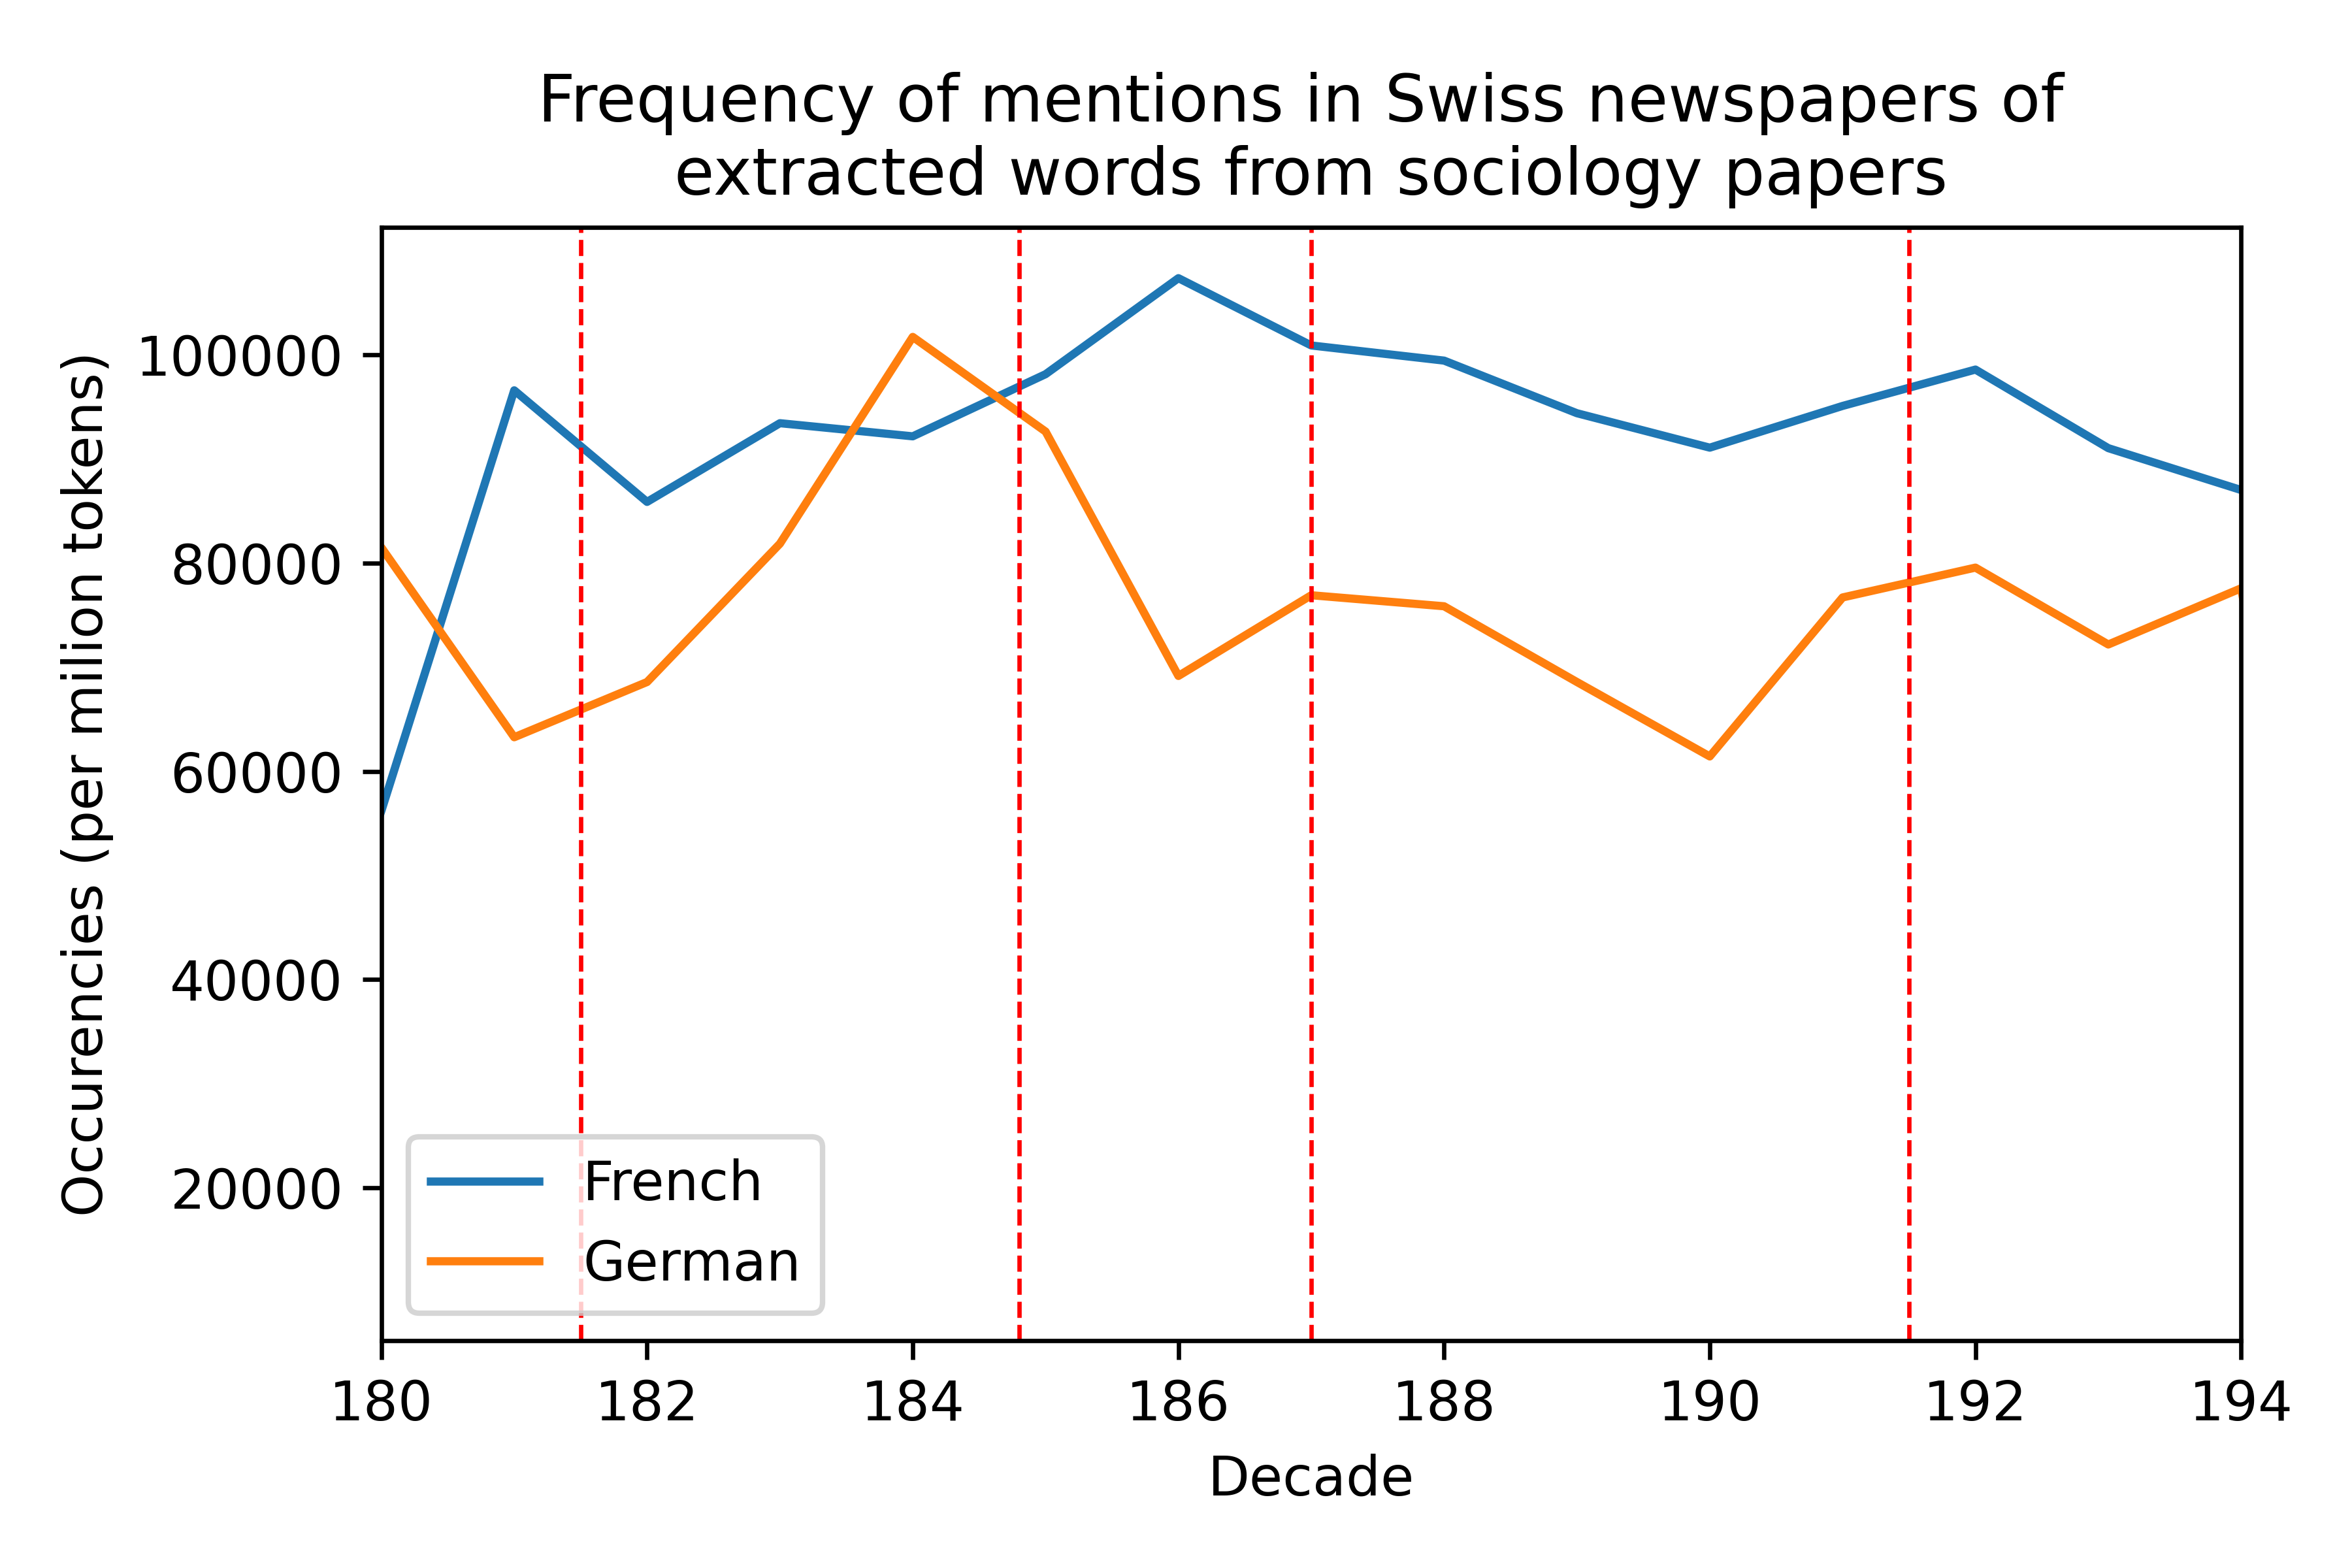
\includegraphics[scale=0.48]{figures/both.png}}
  %  \mbox{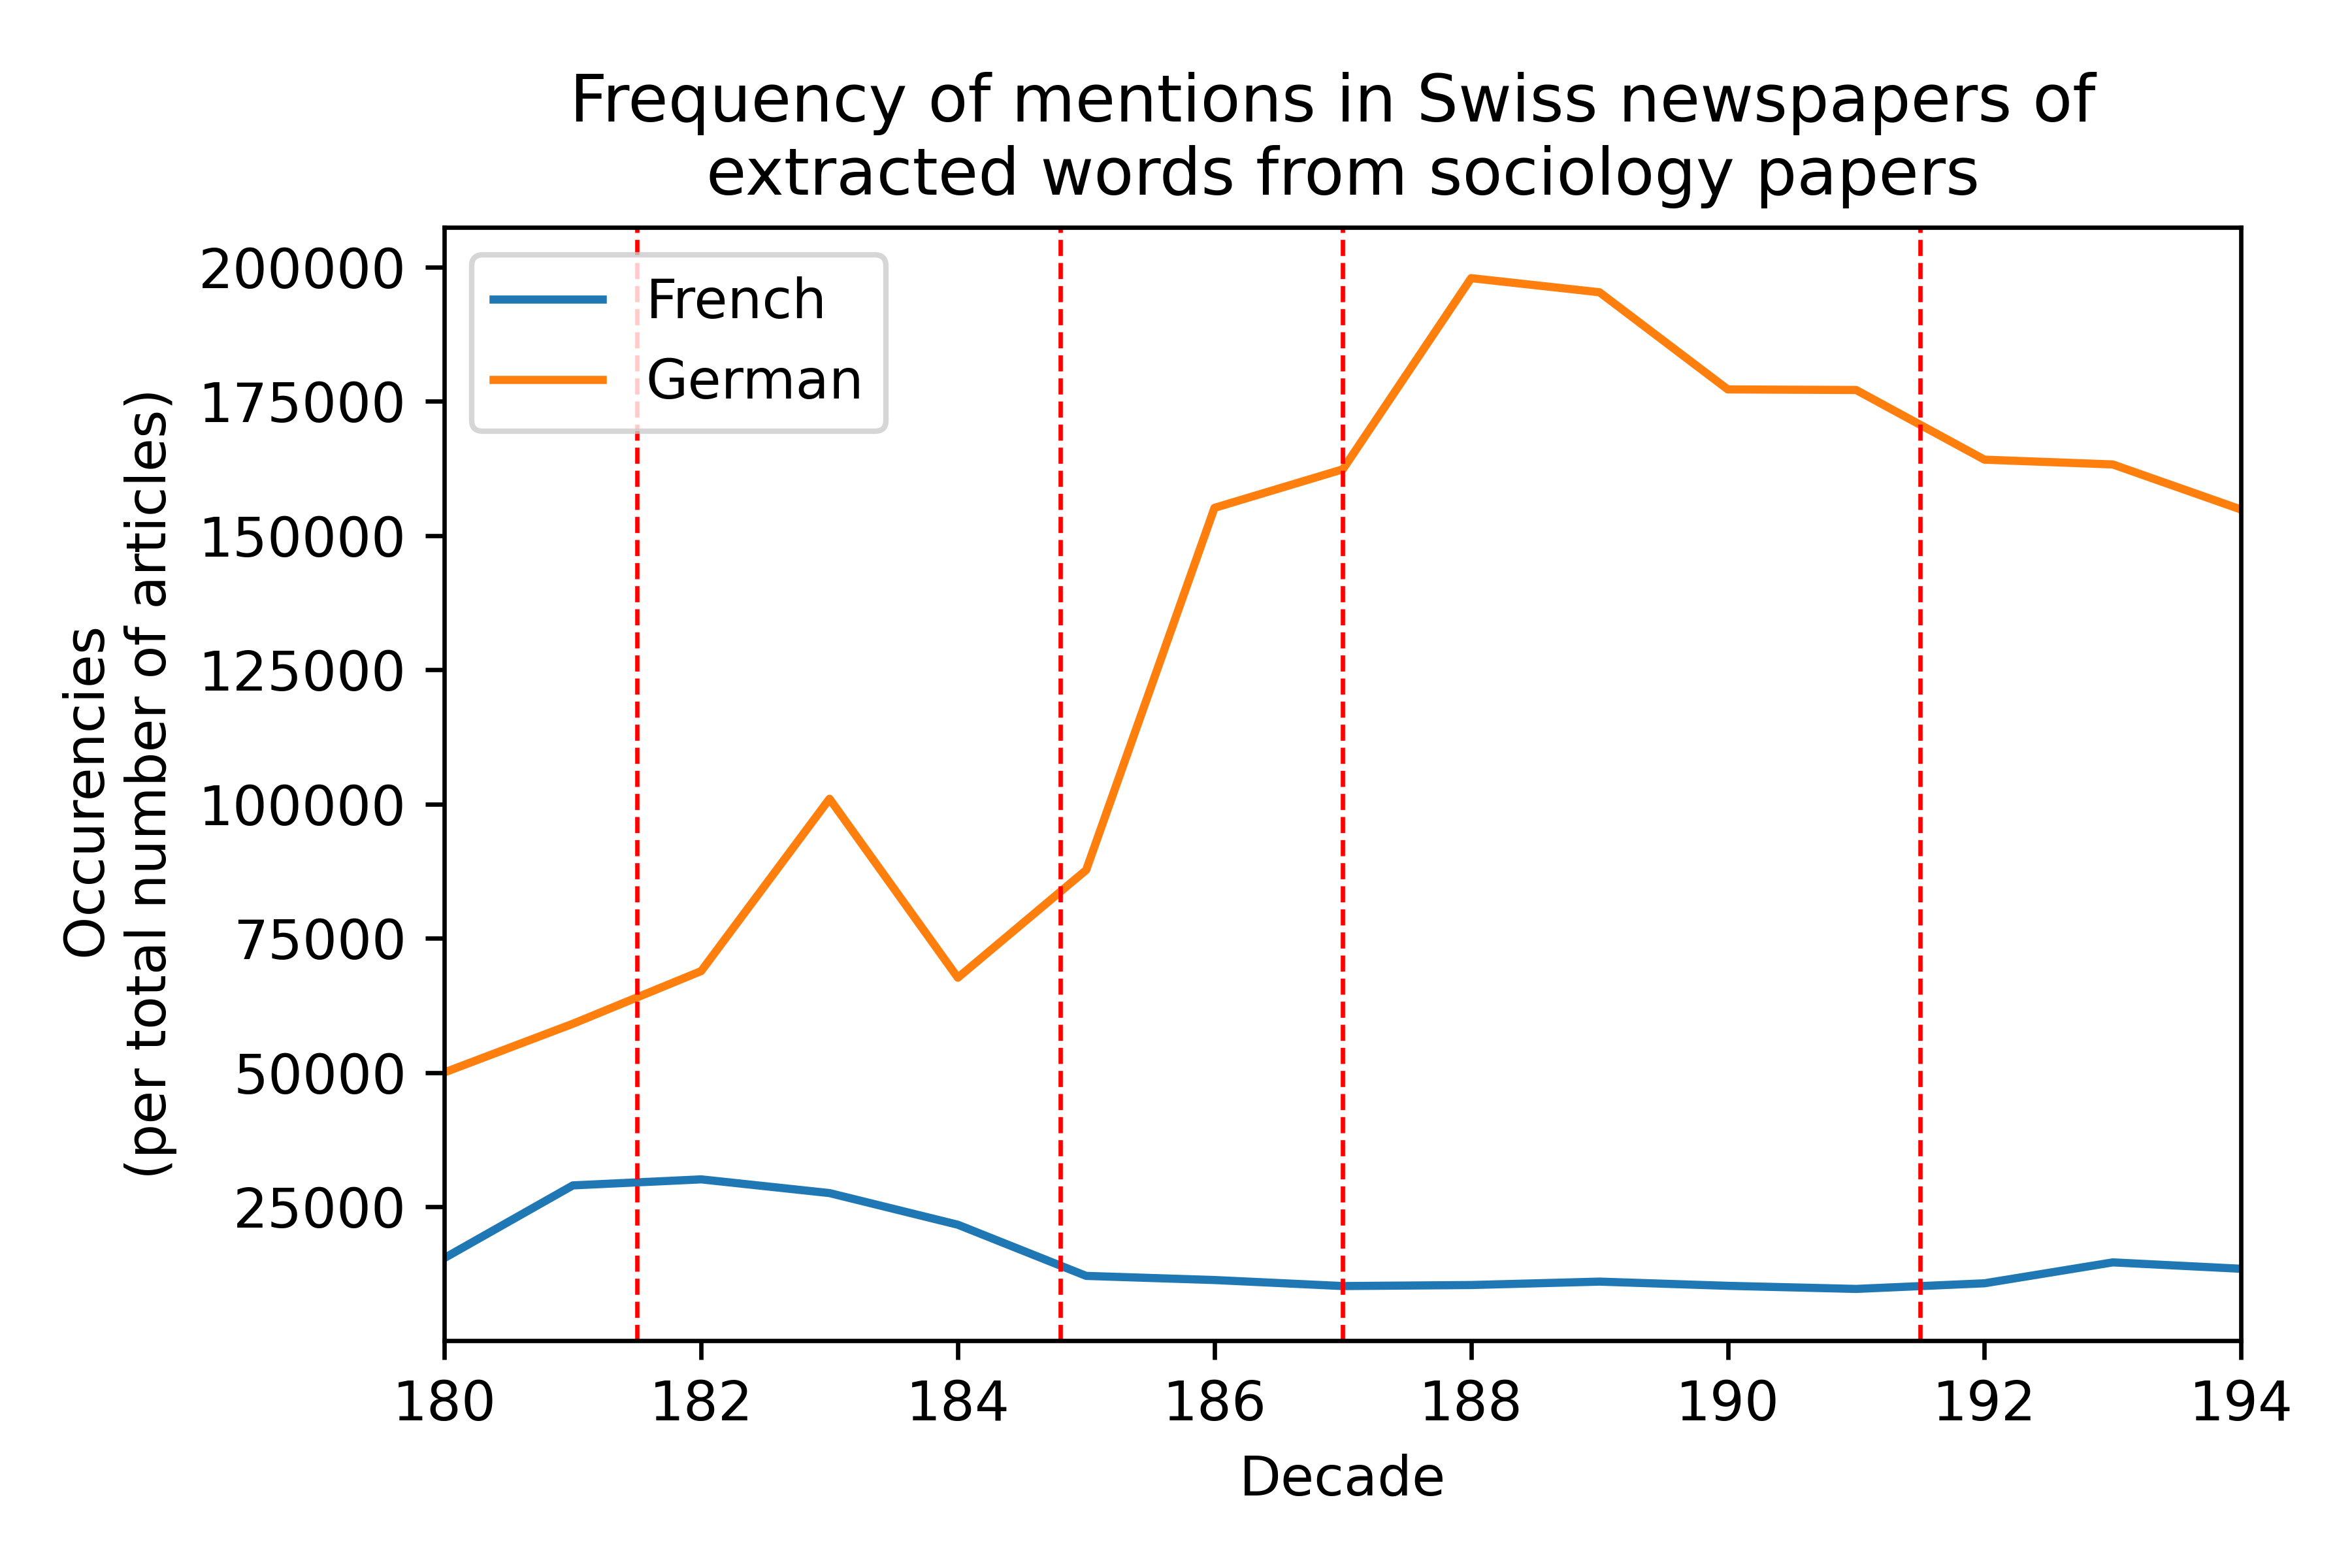
\includegraphics[scale=0.48]{figures/both_normalized.png}}
   % \label{fig:soc_long}
%    \caption{Longitudinal plots. The plot on the left is normalized by million tokens, while the plot on the right by number of articles published in the decade. Vertical lines are drawn for reference at the dates of 1815, 1848, 1870, and 1915.}
%\end{figure}


\newpage

\section*{Appendix 6: TF-IDF results for WW1 propaganda corpus}

\begin{table}[H]
\centering
\small
\captionof{table}{\small Top 50 French n-grams from Swiss newspapers propaganda}\label{propaganda_table_fr}
\begin{tabular*}{\textwidth}{|l|| @{\extracolsep{\fill}} l c || l c |} 
\hline
Rank & Unigram & TFIDF Value  & Bigram & TFIDF Value \\
\hline
\hline
0 & guerre & 0.067719 & conseil fédéral & 0.009438 \\
1 & allemand & 0.041407 & sous marin & 0.008998 \\
2 & monsieur & 0.036717 & etats unis & 0.007338 \\
3 & allemagne & 0.029903 & prisonnier guerre & 0.006319 \\
4 & suisse & 0.028935 & peut être & 0.00614 \\
5 & grand & 0.023987 & autriche hongrie & 0.005965 \\
6 & pays & 0.021985 & état major & 0.005069 \\
7 & gouvernement & 0.021658 & point vue & 0.004928 \\
8 & français & 0.019973 & guerre naval & 0.004837 \\
9 & faire & 0.019232 & grand hôtel & 0.0046 \\
10 & armée & 0.018993 & grande bretagne & 0.004333 \\
11 & france & 0.017375 & début guerre & 0.004253 \\
12 & peuple & 0.016846 & guerre actuel & 0.004251 \\
13 & italie & 0.01648 & prix modérer & 0.004113 \\
14 & devoir & 0.016071 & new york & 0.004089 \\
15 & jour & 0.015745 & austro allemand & 0.004001 \\
16 & paix & 0.015542 & chemin fer & 0.003925 \\
17 & journal & 0.015221 & monsieur venizelos & 0.003809 \\
18 & pouvoir & 0.014947 & temps guerre & 0.003683 \\
19 & politique & 0.014702 & pays neutre & 0.003624 \\
20 & conseil & 0.014508 & croix rouge & 0.003602 \\
21 & général & 0.014501 & déclaration guerre & 0.003577 \\
22 & prendre & 0.014427 & austro hongrois & 0.003437 \\
23 & militaire & 0.01421 & timbre poste & 0.003412 \\
24 & nouveau & 0.013678 & opinion public & 0.003325 \\
25 & fédéral & 0.013583 & affaire étranger & 0.003216 \\
26 & russe & 0.013497 & gazette lausanne & 0.0031 \\
27 & homme & 0.013395 & allemagne autriche & 0.003075 \\
28 & angleterre & 0.013253 & armée allemand & 0.003016 \\
29 & situation & 0.013245 & grand nombre & 0.002943 \\
30 & paris & 0.01312 & gouvernement allemand & 0.002936 \\
31 & ennemi & 0.013098 & commencement guerre & 0.002895 \\
32 & temps & 0.013095 & marin allemand & 0.002888 \\
33 & italien & 0.013045 & monsieur asquith & 0.00284 \\
34 & donner & 0.012983 & maison peuple & 0.002815 \\
35 & neutralité & 0.012851 & impôt guerre & 0.002793 \\
36 & allié & 0.012712 & france angleterre & 0.002785 \\
37 & vouloir & 0.012673 & suisse allemand & 0.002784 \\
38 & août & 0.012645 & président conseil & 0.00278 \\
39 & prisonnier & 0.012458 & confort moderne & 0.002753 \\
40 & etat & 0.012449 & peuple allemand & 0.002737 \\
41 & lausanne & 0.012355 & prix guerre & 0.00272 \\
42 & heure & 0.01234 & champ bataille & 0.002685 \\
43 & anglais & 0.012293 & conseil etat & 0.002661 \\
44 & droit & 0.012208 & gouvernement italien & 0.002644 \\
45 & fr & 0.012092 & sous marin allemand & 0.002635 \\
46 & falloir & 0.011987 & ordre jour & 0.002627 \\
47 & neutre & 0.011826 & guerre aérien & 0.002556 \\
48 & belgique & 0.011674 & emprunt guerre & 0.002522 \\
49 & étranger & 0.01152 & monde entier & 0.002431 \\
\hline
\end{tabular*}
\end{table}

\begin{table}[H]
\begin{small}
\begin{center}
\captionof{table}{\small Top 50 German n-grams from Swiss newspapers propaganda}\label{propaganda_table_gsw}
\begin{tabular*}{\textwidth}{|l|| @{\extracolsep{\fill}} l c || l c |} 
\hline
Rank & Unigram & TFIDF Value  & Bigram & TFIDF Value \\
\hline
\hline
0 & krieg & 0.051574 & vereinigte staat & 0.00819 \\
1 & deutsch & 0.038239 & fr fr & 0.007286 \\
2 & de & 0.030943 & täglich ausgabe & 0.006127 \\
3 & deutschland & 0.025976 & wiener korr & 0.005881 \\
4 & fr & 0.024083 & sept havas & 0.005365 \\
5 & land & 0.021087 & staat deutschland & 0.005331 \\
6 & feind & 0.020704 & oesterreich ungarn & 0.005325 \\
7 & staat & 0.01983 & st galle & 0.004997 \\
8 & stehen & 0.018275 & ausbruch krieg & 0.004683 \\
9 & lassen & 0.017752 & havas amtliche & 0.004646 \\
10 & kriegsschauplatz & 0.017719 & della sera & 0.004543 \\
11 & ge & 0.017484 & neutral staat & 0.004459 \\
12 & england & 0.016757 & deutsch land & 0.004455 \\
13 & bringen & 0.016658 & de krieg & 0.004386 \\
14 & regierung & 0.016263 & amtliche mitteilung & 0.00435 \\
15 & feindlich & 0.016228 & neutral land & 0.004325 \\
16 & finden & 0.016109 & mill fr & 0.004314 \\
17 & front & 0.015792 & deutsch volk & 0.004268 \\
18 & volk & 0.015762 & kriegführend staat & 0.004182 \\
19 & truppe & 0.015605 & wolff amtlich & 0.004144 \\
20 & italien & 0.014835 & öffentlich meinung & 0.003882 \\
21 & telephon & 0.014813 & mai havas & 0.00386 \\
22 & friede & 0.014577 & nov havas & 0.003795 \\
23 & di & 0.014363 & europäisch krieg & 0.003658 \\
24 & dr & 0.014266 & deutsch truppe & 0.003651 \\
25 & nehmen & 0.014261 & deut schen & 0.003635 \\
26 & schweiz & 0.014225 & schwer verlust & 0.003543 \\
27 & bleiben & 0.014214 & prof dr & 0.003486 \\
28 & letzt & 0.014163 & deutsch regierung & 0.003465 \\
29 & ver & 0.01405 & okt havas & 0.00344 \\
30 & frankreich & 0.014037 & kanton zürich & 0.003217 \\
31 & frau & 0.013769 & verfügung stellen & 0.003167 \\
32 & fein & 0.013728 & sept wolff & 0.003117 \\
33 & sehen & 0.013664 & million franke & 0.003074 \\
34 & unb & 0.013524 & frankreich england & 0.00301 \\
35 & havas & 0.013501 & england frankreich & 0.002933 \\
36 & dah & 0.013458 & frau kind & 0.002856 \\
37 & prozent & 0.013296 & deutsch reich & 0.002831 \\
38 & kampf & 0.013272 & beginn krieg & 0.002813 \\
39 & russisch & 0.013191 & italien mailand & 0.002753 \\
40 & sept & 0.013185 & aug havas & 0.002707 \\
41 & armee & 0.012967 & fangen nehmen & 0.002698 \\
42 & stellen & 0.012852 & dr meyer & 0.002656 \\
43 & mai & 0.012786 & deutsch seite & 0.002596 \\
44 & frage & 0.012764 & juni havas & 0.00259 \\
45 & halten & 0.012732 & stadt zürich & 0.002561 \\
46 & geben & 0.01249 & unb bie & 0.002554 \\
47 & liegen & 0.012156 & deutsch österreichisch & 0.002539 \\
48 & leben & 0.01212 & präsident wilson & 0.002533 \\
49 & schwer & 0.012108 & anspruch nehmen & 0.002509 \\
\hline
\end{tabular*}
\end{center}
\end{small}
\end{table}


\newpage

\section*{Appendix 7: Examples of words in context for French and German}

\begin{figure}[H]     
\centering
    \mbox{\includegraphics[scale=0.5]{figures/nationsbildung.png}}
    \mbox{\includegraphics[scale=0.4]{figures/nationsbildung_transcripts.png}}
    \caption{Mention of Nationsbildung in Neue Zuricher Zeitung. Translation by Google: 'Aristocracy the most plump kind of arbitrariness and oligarchy generated, and no wonder is e "therefore, when ta" people focus on all " Weis "stimulates to put an end to it. The legal status and di «nation building have hardly much to« er .. «.»; or whatever is then from the representatives of these senior electors for there "  Education, for spreading the scientific spirit », for Improvement of the Richtsvfitge, for there «Defense and s. f. happen?'}
    \label{fig:nationsbildung}
\end{figure}

\begin{figure}[H]
\centering
    \mbox{\includegraphics[scale=0.5]{figures/naturalisation.png}}
    \mbox{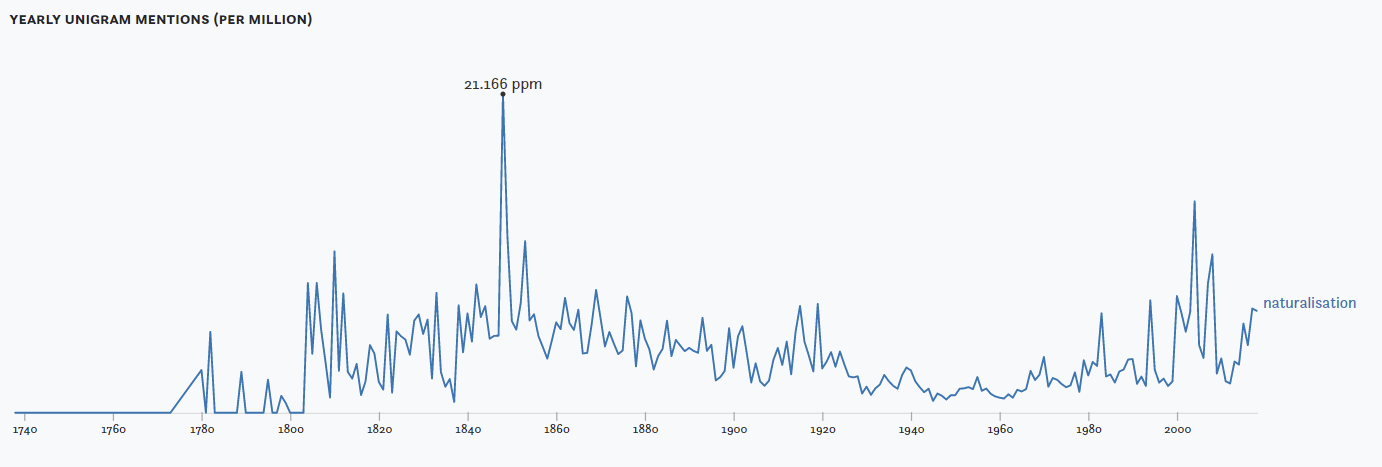
\includegraphics[scale=0.4]{figures/naturalisation_trend.png}}
    \caption{Trend of "naturalisation" occurrences (on the right), with example of occurrence (on the left). Translation of the example: Art. 59. "Is eligible as a member of the national council any secular Swiss citizen with the right to fly. »Swiss citizens who become citizens through naturalization are not eligible only after five years of possession of the right of citizenship. "}
    \label{fig:naturalisation}
\end{figure}

\end{document}



The XIX century in Europe is, among others, defined by the emergence of the nation state as exemplified by  the German (1871), Italian (1870) and Swiss nation (1848). Whereas the French, English, German or Italian nations emerged either given a preceding dynastic power over a given geographic territory or a common language, ethnicity and culture  \footnote{"Tantôt l'unité a été réalisée par une dynastie, comme c'est le cas pour la France ; tantôt elle l'a été par la volonté  directe  des  provinces,  comme  c'est  le  cas  pour  la  Hollande,  la Suisse,  la  Belgique ;  tantôt  par  un  esprit  général,  tardivement  vainqueur des  caprices  de  la  féodalité,  comme  c'est  le  cas  pour  l'Italie  et  l'Allema-gne." \citep{renan1882qu}}, Switzerland constitutes a special case\footnote{"Comment  la  Suisse,  qui  a  trois  langues,  deux  religions,  trois  ou  quatre races, est-elle une nation" \citep{renan1882qu}}. \par
For most its history, Switzerland was a loose federation of different city-states or small independent regions bound together by a military union called the Swiss confederation. Thus, for a long time, Swiss people rather identified with their local region, canton or even city than with the Swiss confederation. \par
However, in the last two centuries a Swiss identity arguably emerged, aided by common military service, education, especially historical education, and by common values. This “growing together” was manifested also in the growth in central authority (implementation of national pension schemes and inter-cantonal transfers; \cite{ladner2018schweizer}) . \par
Due to their exceptional stance, Swiss nationalism and national identity have been discussed by a rich body of literature from different scientific communities. 
In our analysis, we would like to contribute to this general discussion by tracing the evolution of Swiss national identity from the 19th century using computational methods. Specifically, we take into consideration the period from the 1820s to the 1950s, when the formation and development of the modern Swiss Nation took place. The goal of this analysis is to articulate the concept of Swiss nationality in a computer understandable manner and to scan the huge corpus of regional Swiss newspapers for its evolution in time. Newspapers have been chosen as they largely reflect and model the opinions and topics of interest to the regional population. The adoption of newspapers as primary source, to the best of our knowledge, has not yet been considered in the analysis of Swiss nationality and could hopefully provide new insights into the matter. \par
The investigation will be comprised of two parts: the extraction of expressions that identify Swiss identity, and the temporal evolution of how these expressions were used in the selected newspapers. For the extraction, we adopt several textual sources that can serve as proxies of national identity. Those proxies are: 1) Early Swiss history books. 2) World War I propaganda articles in newspapers. 3) Political sociology papers on (Swiss) nationalism. Although all presented proxies are inherently biased, by looking at the question from several angles and by taking different proxies into account, this paper aims to produce meaningful and robust results.\par

\section{Context}

Following, this paper presents the historical and sociological discussion surrounding the special case of the Swiss nation and the Swiss identity, which motivates this project and its methodology. Furthermore, the presented sources carry different definitions of Swiss identity and can thus be used to extract meaningful terms, which define Swiss identity throughout the century. In practice, this project uses two history books\footnote{\cite{MuellerJohannes1780} and \cite{seippel1900schweiz}}, World War I propaganda articles published in Swiss newspapers, and several sociological papers which deal with Swiss identity to extract 'Swiss identity terms' as it will be described in the Methodology. 

\subsection{Swiss History}
The modern Swiss nation arguably emerged from a complex construct of treaties and inter-regional dependencies commonly referred to as the 'Swiss Confederation' \citep{Eidgenossenschaft_hsl_2012}. The members of this confederation were bound together by a multitude of contracts \footnote{The oldest still existing contract dates back to 1291}. \citep{Bundesbriefe_hsl_2012}.\par
Those medieval contracts and treaties often opposed the influence of surrounding European powers (especially the France and the Hapsburg) while reinforcing economic links between the Swiss regions. 
Those early contracts between the members of the Swiss confederation would be reinterpreted by early historians as a common endeavour for self government, autarchy and self determination of the individual Swiss regions (see 'Chronicon Helveticum' \cite{tschudi1734chronicon}.\par
In the 18th century, nationalistic forces driven by the spirit of the enlightenment used a similar narrative to solidify their case for a unified Swiss nation. Extending on it by claiming that the Swiss people  must be considered an homogeneous ethnicity\footnote{The so called 'helvetics', populating the central alps} and thus belong in a common nation (see 'The history of the Swiss confederates' \cite{MuellerJohannes1780}. \par
This ethnic understanding of the Swiss nation was deeply questioned at the end of the 19th century.
Historians increasingly argued that the concept of 'the Swiss nation and it's people' was created during the 19th century aided by national institutions as common military service, national celebrations, national societies and a common myth of origin (see \cite{seippel1900schweiz} and \cite{renan1882qu}). \par

The two world wars asserted again the importance of a common Swiss national identity. During this time, the central government and military leadership allocated considerable resources to solidify Swiss patriotism, in an act which would be referred to as 'spiritual defense'. This ideology stated that Switzerland in its cultural and ethnic diversity was unified by a common set of beliefs and a 'spiritual unity'\footnote{"L'idée  suisse  n'est  pas  un  produit  dela  race,  c'est-à-dire  de  la  chair,  mais  une  œuvre de  l'esprit.  C'est  un  faitadmirable  qu'autour  du  Gothard,  montagne  qui  sépare  et  col  qui  unit,une grande idée,  une idée européenne, universelle, ait  pu prendre naissanceet  devenir  une  réalité  politique:  l'idée  d'une  communauté  spirituelle  despeuples  et  des  cultures  occidentales." (P. 1012, \cite{conseilFederal1938})}. \citep{LandesverteidigungJorio_hsl_2012} \par 
In practice, for extracting Swiss identity from Swiss history books the works of \cite{MuellerJohannes1780} and \cite{seippel1900schweiz} in French and German language have been used. 

\subsection{Political Sociology of Nation}
Many influential authors addressed the 'Swiss case' as that edge case that could confirm or dismiss their theory on Nationhood. Among others, the names of Anderson, Renan, Weber, Kohn appear in the long list (\cite{wimmer2011swiss}). 
\par

According to \cite{wimmer2011swiss}, Switzerland is a case of multi-ethnic nation, where even cantonal borders are independent of language borders. However, even considering Switzerland multi-ethnic has been widely questioned and numerous other options have been put forward. Switzerland has been considered post-national, multi-national, quasi-ethnic and much more \citep{helbling2011switzerland}. Alongside the problematization of its definition as a nation, \cite{wimmer2011swiss} and \cite{helbling2011switzerland} show how major theorists differ widely in their explanation on the nature and foundation of Swiss nationality: Weber \footnote{\citep{weber1978economy}} sees Switzerland as an example of how a nation can be based on commonality of political spirit rather than objective attributes. For Kohn \footnote{\citep{kohn1956nationalism}} and Deutsch \footnote{\citep{deutsch1953nationalism}}, the republican regime and the advanced communication channel created the cohesion of this nation despite its lack of common cultural background. Gellner \footnote{\citep{gellner1991nationalisme}, \citep{gellner2008nations}} argues that the Swiss nation can only be explained taking into account the extremely high level of literacy, which removes the need for a shared language. 
Based on the above theories, \cite{wimmer2011swiss} identifies the creation of the Swiss national concept in the bourgeois associations that formed in the XVII century. These associations aimed at a progressive union and equality between rural and urban areas. Those societies proclaimed a 'community of progress' that was meant to disseminate the national sentiment. This was done based on republican and liberal ideals rather than nationalism itself.

Overall, the Swiss case can be well explained as a process shaped by a changing social context, where the will of the people (Willensnation) and the natural communion of the different ethnicities (Wesensgeheimschaft) forged Switzerland as a nation \citep{zimmer1999forging}. The first entails a political action, where some key actors form the Swiss concept of nation and the population follows, the second is the ensemble of pre-existing indigenous folk traditions, myths, symbols, narratives and
beliefs, which distinguish the Swiss from the outside \citep{zimmer1999forging}. \par

Lastly, it is important to keep in mind the pivotal accounts given by Anderson and Renan. The first envisages nation as “an imagined political community [...] It is imagined because the members [...] will never know most of their fellow-members [...], yet in the minds of each lives the image of their communion (p.2)” \citep{anderson2006imagined}. Switzerland is, therefore, a nation in virtue of the imagination of its members to belong to the same nation. According to \cite{renan1882qu} the nation is a "spiritual principle" based on a common past and heritage. In line with this theory, the Swiss proclaim themselves Swiss given their common past.
\par
To create the corpus for extraction, the papers cited by \cite{wimmer2011swiss} and \cite{helbling2011switzerland} and written in either French of German were searched for (i.e. \cite{imhof1993nationalismus}). Since not all of those were publicly available, papers citing the major theorists were also downloaded whenever possible (i.e. \cite{godechot1971nation}). Attention was payed to retrieving both older, foundational papers (from the 1960s-1990s) and more recent ones (XXI century). Moreover, both papers discussing specifically the Swiss case and those introducing a general theory of nationalism were included. Finally, texts pertaining from different theories (subjectivist, objectivist, ...) were retrieved. The full list of papers gathered can be found in Appendix 1. 

\section{Data}

For the analysis, data are used with two purposes: extracting expressions on Swiss identity and tracing the expressions in time in newspapers. Regarding the first use, the three types of sources were already mentioned in the Research Context. The texts mentioned are retrieved in .txt format, and they consist of two history books, newspapers containing propaganda, and 18 political sociology papers. Most of these resources are retrieved from the Swiss National Library, French National Library (Gallica), Google Books, and E-Periodica. \par

Each of the three types of sources is associated a reference corpus, to be able to extract TFIDF scores by computing an inverse document frequency. A suitable reference corpus for Swiss historical literature in French and German is provided in the 'Trés Grand Bibliotheque' \citep{TresGrandBibliotheque} and in the 'Deutsches Textarchiv'\citep{DeutscheTextArchive}. For WW1 propaganda newspapers, a sample of 10000 articles from the Swiss press, published in the two major newspapers in the period before the WW1 (1901-1914) serves as a reference, assuming there was no need for national propaganda before the war had started. For sociology articles, a corpus of papers published in JSTOR sociology journals between 1960-2020 in French (and containing the word sociologie) and in German (and containing the word Soziologie) is used. \par

In terms of the second use, this project adopts a large scale corpus of different regional newspapers, the Impresso Platform, by \cite{Ehrmann2020LanguageRF}. The Impresso project gathered and pre-processed an impressive corpus of over 36 millions articles from diverse set of Swiss newspapers. To our best knowledge, it is the biggest data set which can be easily used to analyse Swiss newspapers over the XIX and XX century. An exploratory analysis has shown that a reasonable amount of data is available in two out of the four Swiss national languages: French and German.\par
Finally, only the Gazette de Lausanne and Neue Zuricher Zeitung were used as these are two local newspapers representative of their regions, issued in the capitals of the cantons with the biggest french-speaking and german-speaking population. 


\section{Methods}
As for the Data, the Methodology is composed of two steps: a TFIDF n-gram extraction from the corpora on Swiss identity and a longitudinal analysis of the frequency of the extracted unigrams over the two selected journals in the Impresso Platform. \par

From the three corpora gathered (as described in the sections above), pre-processing steps were applied in order to obtain a clear extraction: the texts were tokenized, stopwords were removed and POS (Part of Speech) tagging was used to maintain only adjectives, adverbs, nouns, pronouns and verbs (as we consider those the most informative parts of sentence). Furthermore, lemmatization was used to reduce terms to their word stem.\par
Following, the TFIDF scores were computed for 1-grams to 4-grams, where the inverse term frequencies were computed against reference corpora, and the resulting weights for each word were determined as follows:
\[w_{i,j} = tf_{i,j} \cdot log(\frac{N}{df_{i}})\]
where $w_{i,j}$ is weight of the word $i$ in document $j$, the $tf_{i,j}$ is the number of occurrences of $i$ in $j$, $N$ is the number of documents and $df_{i}$ is the number of documents containing the word $i$. \par

Each of the types of sources was considered as one document and compared against all the documents in the corresponding baseline corpus. The 50 unigrams with the highest resulting weights for each type of source were then used in the n-gram frequency analyzer in the Impresso Platform\footnote{The tool can be found \href{https://impresso-project.ch/app/search/ngrams?sq=ChYIARACGAcgASoMbmF0aW9uYWxpc21l}{here}}. The previous work of \cite{Twenge2012IncreasesII} shows that the quantitative analysis of the word frequency in time on the large corpora can unveil the trends, not only in language, but also in the changing society and public opinions. With this purpose in mind, this project uses the extracted words to show how their aggregated yearly trends of use fluctuated through time. Once the words are plugged in, the tool scans through all the OCRed corpus and calculates the aggregated frequency in time for the selected n-grams, in absolute values, and as a ratio per milion tokens. Some filtering is applied before the search: only articles in French and German, that were published in Switzerland in either Gazette de Lausanne or Neue Zuricher Zeitung were selected.  

Finally, the frequency per million tokens of all the 50 unigrams is aggregated and plotted in time with a running mean of a decade. The resulting plots can be observed in the Results section. 

\section{Results}
\subsection{History}
By using the historical works of \cite{MuellerJohannes1780} and \cite{seippel1900schweiz} and comparing them with the aforementioned reference corpora with the TFIDF method, we obtain the term list presented in Appendix \ref{appendix4}. \par
\begin{table}[H]
\small
\begin{scriptsize}
\centering
\caption{Selected terms, Swiss history}\label{TFIDF_Terms_Top_Twenty_desc}
\begin{tabular}{|l|l|l|} 
\hline
Self identified Topic & German terms & French  terms  \\
\hline
\makecell{Swiss places  \\ or nation} & \makecell{zürich  / luzern / bern /  waadt / z̈urich bern / schweiz  \\ eidgenossenschaft / helvetien / helvetischen republik } & \makecell{berne /  zurich / bernois / schwyz  \\ suisse allemand  / suisse /  alliance }  \\
\hline
\makecell{Significant people in \\ Swiss history} & \makecell{numa droz  / bonaparte / general bachmann  } & \makecell{comte pierre /  rodolphe habsbourg / abbé saint-gall \\ empereur fŕed́eric /  jean bubenberge } \\
\hline
European powers   & \makecell{französisch  / frankreich / franz̈osisch gesandte \\ schweiz frankreich / franz̈osisch truppe } & \makecell{habsbourg /  empereur / savoie / maison habsbourg \\ empereur fŕed́eric  / habsbourg lauffenbourg }  \\
\hline
\makecell{Political institutions} & \makecell{tagsatzung / partei / behörde / verfassung \\ bürger / öffentlich / republik / volk \\ öffentliche meinung / volks nah \\ demokratischer kanton / neutralität schweiz } & \makecell{ bourgeois / charte  / alliance / frère \\ bourgeois berne/ traité paix /  électeur mayence } \\
\hline

\hline
\end{tabular}
\end{scriptsize}
\end{table} 
Analysing the obtained German and French terms, one can identify recurring themes expressed by a group of terms which seem to describe the same concepts. Many of those identifiable themes occur in the German as well as in the French term lists.  \par 
A first striking and intuitive topic seems to be the mentioning of Swiss cantons, cities and places or the Swiss nation itself. This topic seems to be a rather intuitive result due to the chosen TF-IDF method, given that the comparative corpora probably rarely contain books which discuss Switzerland or Swiss cities. The three different term used to name Switzerland (e.g.: Schweiz, Eidgenossenschaft, Helvetik) correspond to names for Switzerland during different historical periods and already might imply the multifaceted nature of the Swiss identity throughout history. Furthermore, it is also interesting to analyse the cantons, cities and places which are mentioned and on the other hand the places which are not mentioned. Here one could for example state that the historical rivalry between and the importance of Bern and Zürich is clearly visible given the high TF-IDF values of both cities and  given the fact that there is even a bigram ‘Zürich Bern’. \par
A similarly intuitive theme is the frequent mentioning of people, which might be in some sense significant for Swiss history. The most important bigram for the German list, for example, is the name Numa Droz, who was an influential Swiss politician and one of the first members of the federal council. The French list refers, multiple times, to Rodolphe Habsbourg, who was a medieval ruler who repeatedly waged war against the Swiss confederation. The French term list also mentions Whilhelm Tell (Guillaume Tell), who reportedly rebelled against the Habsbourgs. \par
Another related and dominant theme visible in the term lists, is that of foreign European powers. This might substantiate the fact that the surrounding European powers deeply influence the creation of the Swiss nation, as already discussed in the literature part. Interestingly, comparing the French to the German term list it is notable that, while the French list mostly mentions the Habsburgs, the German term list rather tends to mention the French empire. This is most probably the result of the different reference corpora, given that the French reference corpus is more likely the discuss French history, while the German reference corpus rather discusses the history of the German empires.  \par
A last notable theme discusses Swiss political institutions and principles. This topic is more ambiguous and mentions terms like the government, the constitution, the public, the people, the military and neutrality. Although many of those words have a very strong connotation in discussing Swiss identity, it still seems interesting that the obtained words describe rather abstract concepts. Furthermore, the German and French list also do not seem to be always consistent. For example, where as the French list several times mentions the Bourgeois (of different cities) the German list only mentions the people (e.g.: Volk, volksnah, bürger). \par
Using the top 50 French and German uni-grams and inputting them into the Impresso frequency analyser, we obtain the time series presented in Figure \ref{fig:cumulative_history}.The time trend of the mentions of the obtained Swiss history terms, reveals an interesting pattern with peaks corresponding to important historical events, as marked by the red dotted lines in Figure \ref{fig:cumulative_history}. The selected historical dates signify instances during which the Swiss nation was either questioned or crucially influenced by external events. Thus the peaks in the usage of the Swiss history terms, might have been caused by the newspaper journalists reflecting upon Swiss identity during those historically significant times. 
Furthermore, comparing the trend in usage of German terms to the usage of the French terms, it can be observed that the German trend line is more accentuated and better defined by the proposed historical events. \par
In general, the obtained terms seem to be an intuitive representation of the two selected books and considering the obtained time trend they seem to encode some notion of Swiss identity.




\begin{figure}[H]
    \centering
    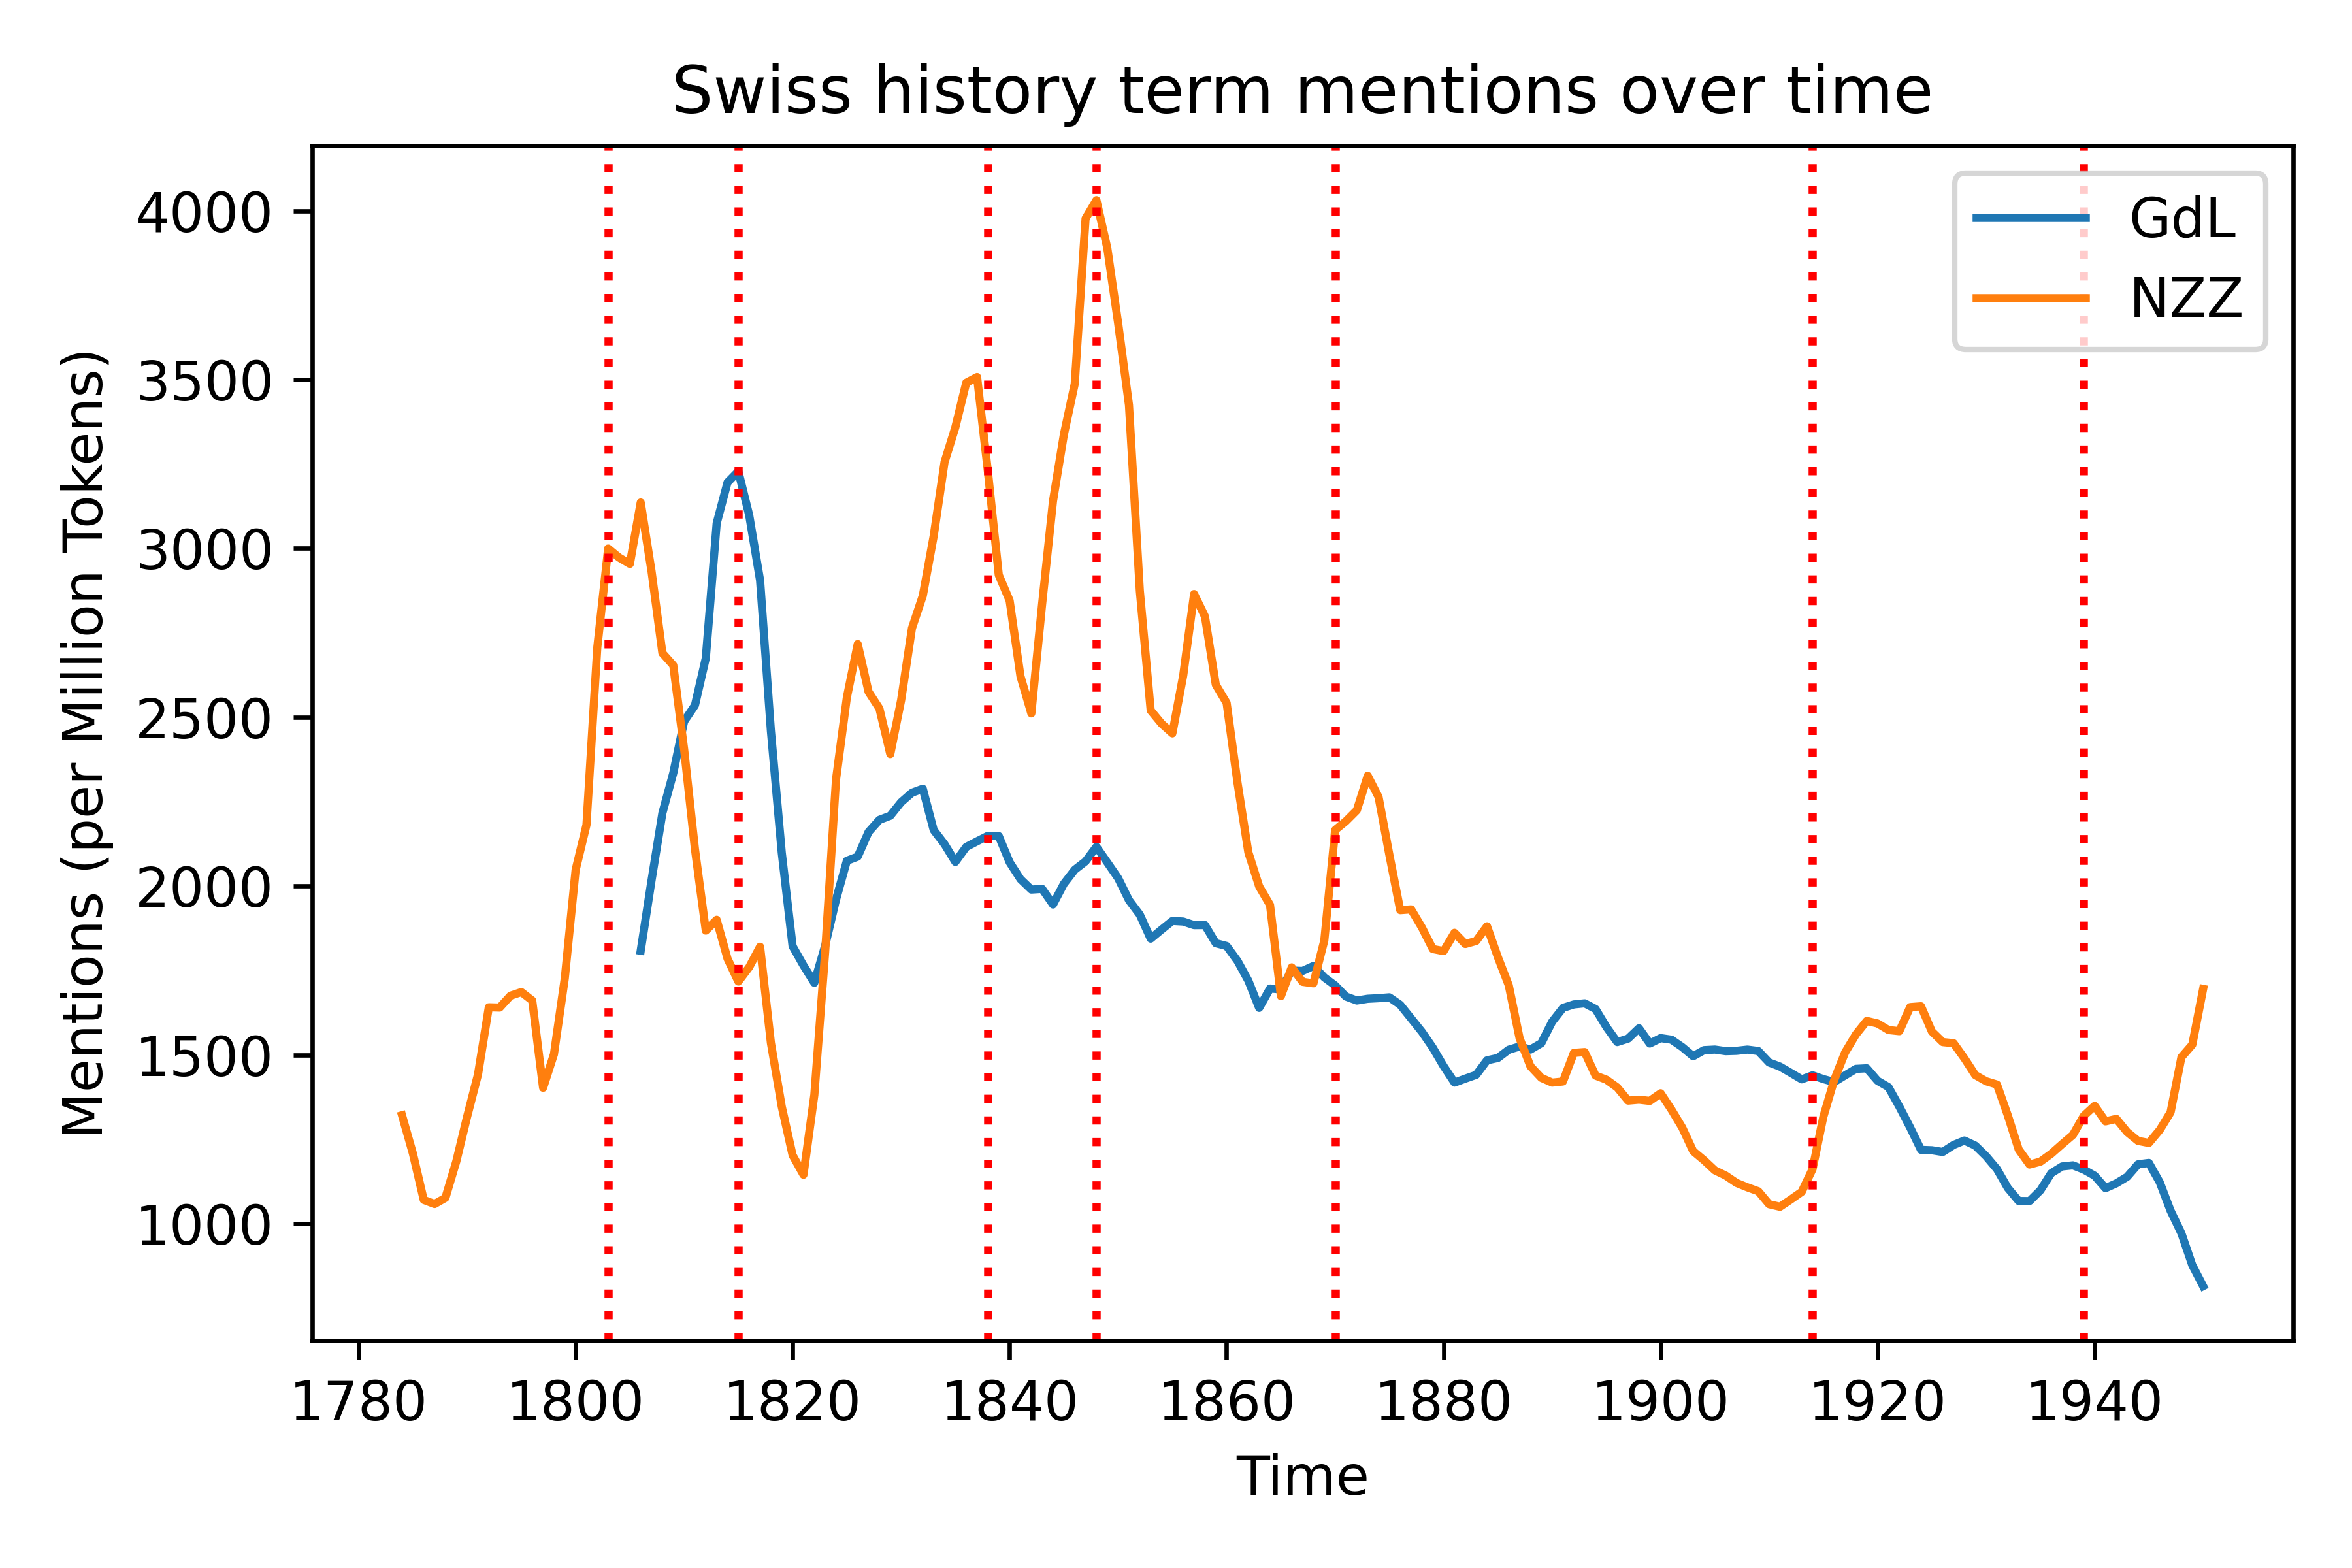
\includegraphics[width=1\linewidth]{figures/History_swiss_identity.png}
    \caption{Longitudinal analysis of cumulative frequences of the 50 most important TF-IDF tokens in the corpus. The red lines represent important historical events:
Mediation under Napoleon (1803), Congress of Vienna (1815), Diplomatic conflict between Swiss confederacy and France (1838), Creation of modern Switzerland (1848), Creation of Italy and Germany (1870), Beginning of I. World War (1915), Beginning of II. World War (1939).
}
    \label{fig:cumulative_history}
\end{figure}




\subsection{Political Sociology}
The n-grams extracted from the political sociology sources are reported in Appendix 5. The extraction, mirroring the focus of the sources, shapes a concept of national identity based on the role of community, state politics, and of construction (or invention) of shared values\footnote{Some words that are particularly representative of this vision are 'convention', 'droit', 'etat',  'politique', 'patrie', 'culture', 'tradition', 'peuple', 'inventer', 'sentiment',  'politisch', 'staat', 'geschichte', 'politische', 'reich', 'einheit', ..}. In particular, the terms extracted delineate a concept of nation that is biased towards a cultural representation, where the nation is voluntary (the already mentioned concept of Willensnation). \par
The words for the French and the German extraction appear radically different. This is motivated by the sources, as the words are likely to encode aspects inherent to the two countries of Germany and France, other than only Switzerland. Assuming this, the words can be interpreted in terms of how the two sets can be used to create a, partial, interpretation of the Swiss nation as seen under the influence of the neighboring countries. In this sense, we analyze the resulting words in terms of how, and to what extent, the conveyed socio-political representation of the national identity of the two neighboring nations can be used to model the share of Swiss identity that is a projection of its neighbors. \par
Looking at the expressions extracted from the French corpus, the representation of nation appears rather abstract \footnote{sens, sentiment, identité, definition, volunté}. The concept is tightly linked to words referring to a patriotic feeling\footnote{patrie, patriotisme, patriote}, which is a characteristic aspect of French Nationalism and French Revolution. This is also important in the Swiss case, that witnessed a rise of patriotism around the 1760s and a boom during the French Revolution (\citep{zimmer1999forging}). Swiss patriotism was funded upon the invocation of a glorious past, and the veneration of memory of the Swiss Confederation of the 14th and 15h century. Among the French words, a great deal of importance is given to the n-grams representing nationalist thinkers and theories. Among these, the aforementioned 'imagined community' by Anderson figures in the top 50 list, and an ever greater resonance can be seen in the bigram 'invented traditions’. The expression was coined by Hobsbawm and it indicates the action of the nationalist elites who shape and construct the way in which nation enters the public discourse (\citep{anderson2006imagined, hobsbawm2012invention}). In this view, public rituals, ceremonies, and national symbols are nothing more than utilitarian inventions of those striving to create the nation. In line with the patriotic nature of Swiss nationalism, this view mirrors the large effort of creation of Swiss identity by means of myths and symbols, which culminated in the ceremonies of celebration of the Swiss nation of 1891 and 1937 (\citep{zimmer1999forging, wimmer2011swiss}). \par
Transitioning to the German words, attention is given, contrarily, to both abstract aspects and physical ones. We see the appearance of temporal terms\footnote{19 jahrhundert, hälfte 19, französische revolution, 20 jahrhundert}, indicating greater focus on the temporal evolution of the concept in the German corpus; but also terms referring to cultural and sportive activities such as singers and gymnast movement\footnote{sängerbewegung and turnbewegung}. As it becomes evident by the excessive use during the Nazi and Fascist regimes, attention to sportive activities is a profound source of national sentiment, rooted in the political aesthetics of the performance \citep{rossol2010performing}. Many terms, moreover, refer to the military\footnote{militärisch, krieg, stark}, yet another a symbol of national power and pride. Both sportive activities and military are elements at the root of Swiss identity, as epitomized by the Olympics and the pride put into the military system \citep{seippel1900schweiz}. The German words acquire a rather socialist and constructivist connotation, stressing the importance of the volk and of the social sphere, positing attention to the act of Nationsbildung (nation-building), which morphologically implies a concept of nation that has to be constructed by the population. \par
Altogether, the two words extractions define the Swiss nation as a Willensnation based on common ideals and values but also regulations. The most frequent regulations are nationality law\footnote{nationalitè droit, distinguishing citizenship from statelessness}, and naturalization\footnote{naturalisation}. This latter, morphologically based on the latin natura (nature, natural state) is, counter-intuitively, the acquisition of the nationality and the formal entrance in the social state. In the Swiss nation, naturalization is based on normative elements as well as on values\footnote{'The applicant must be well integrated, The applicant must be familiar with life in Switzerland, The applicant must not endanger Switzerland's interior or exterior security, The applicant must show respect for public order and security, The applicant must respect the values of the federal constitution, The applicant must be able to communicate in a national language, both orally and in writing, The applicant must participate in the economy or be in education, The applicant must, if married, in a registered partnership, or a parent, encourage and support the integration of his or her spouse and/or minor children' from Wikipedia on Naturalisation}. This is one of the driving words in the longitudinal plot in \ref{fig:cumulative_sociology}, peaking in frequency on 1848 (see Appendix 7). This often resonates with articles citing or explaining the constitution (as can be seen again in Appendix 7), which explains the peak in attention in 1848, year of publication of the Swiss constitution. 

Looking more generally at the aggregated trend in Figure \ref{fig:cumulative_sociology}, high resonance is achieved around 1848 and coinciding with the official creation of the nation. However, even higher frequencies can be found for the French part right before the Diplomatic conflict between the Swiss and French (in 1838) and before the completion of the nationalist movements in Italy and Germany. The trend seems, therefore, to be anticipating international events, indicating a public discourse about nationalism in the French speaking part in conjunction with conflicts in/with the neighboring countries. The trend for the German is instead reaching maximum resonance during the World Wars, where, as expected, the military and cultural symbols of the nation, which were predominantly extracted in the German words, were mentioned frequently to invoke a Swiss spirit during the wars. 


\begin{figure}[H]
    \centering
    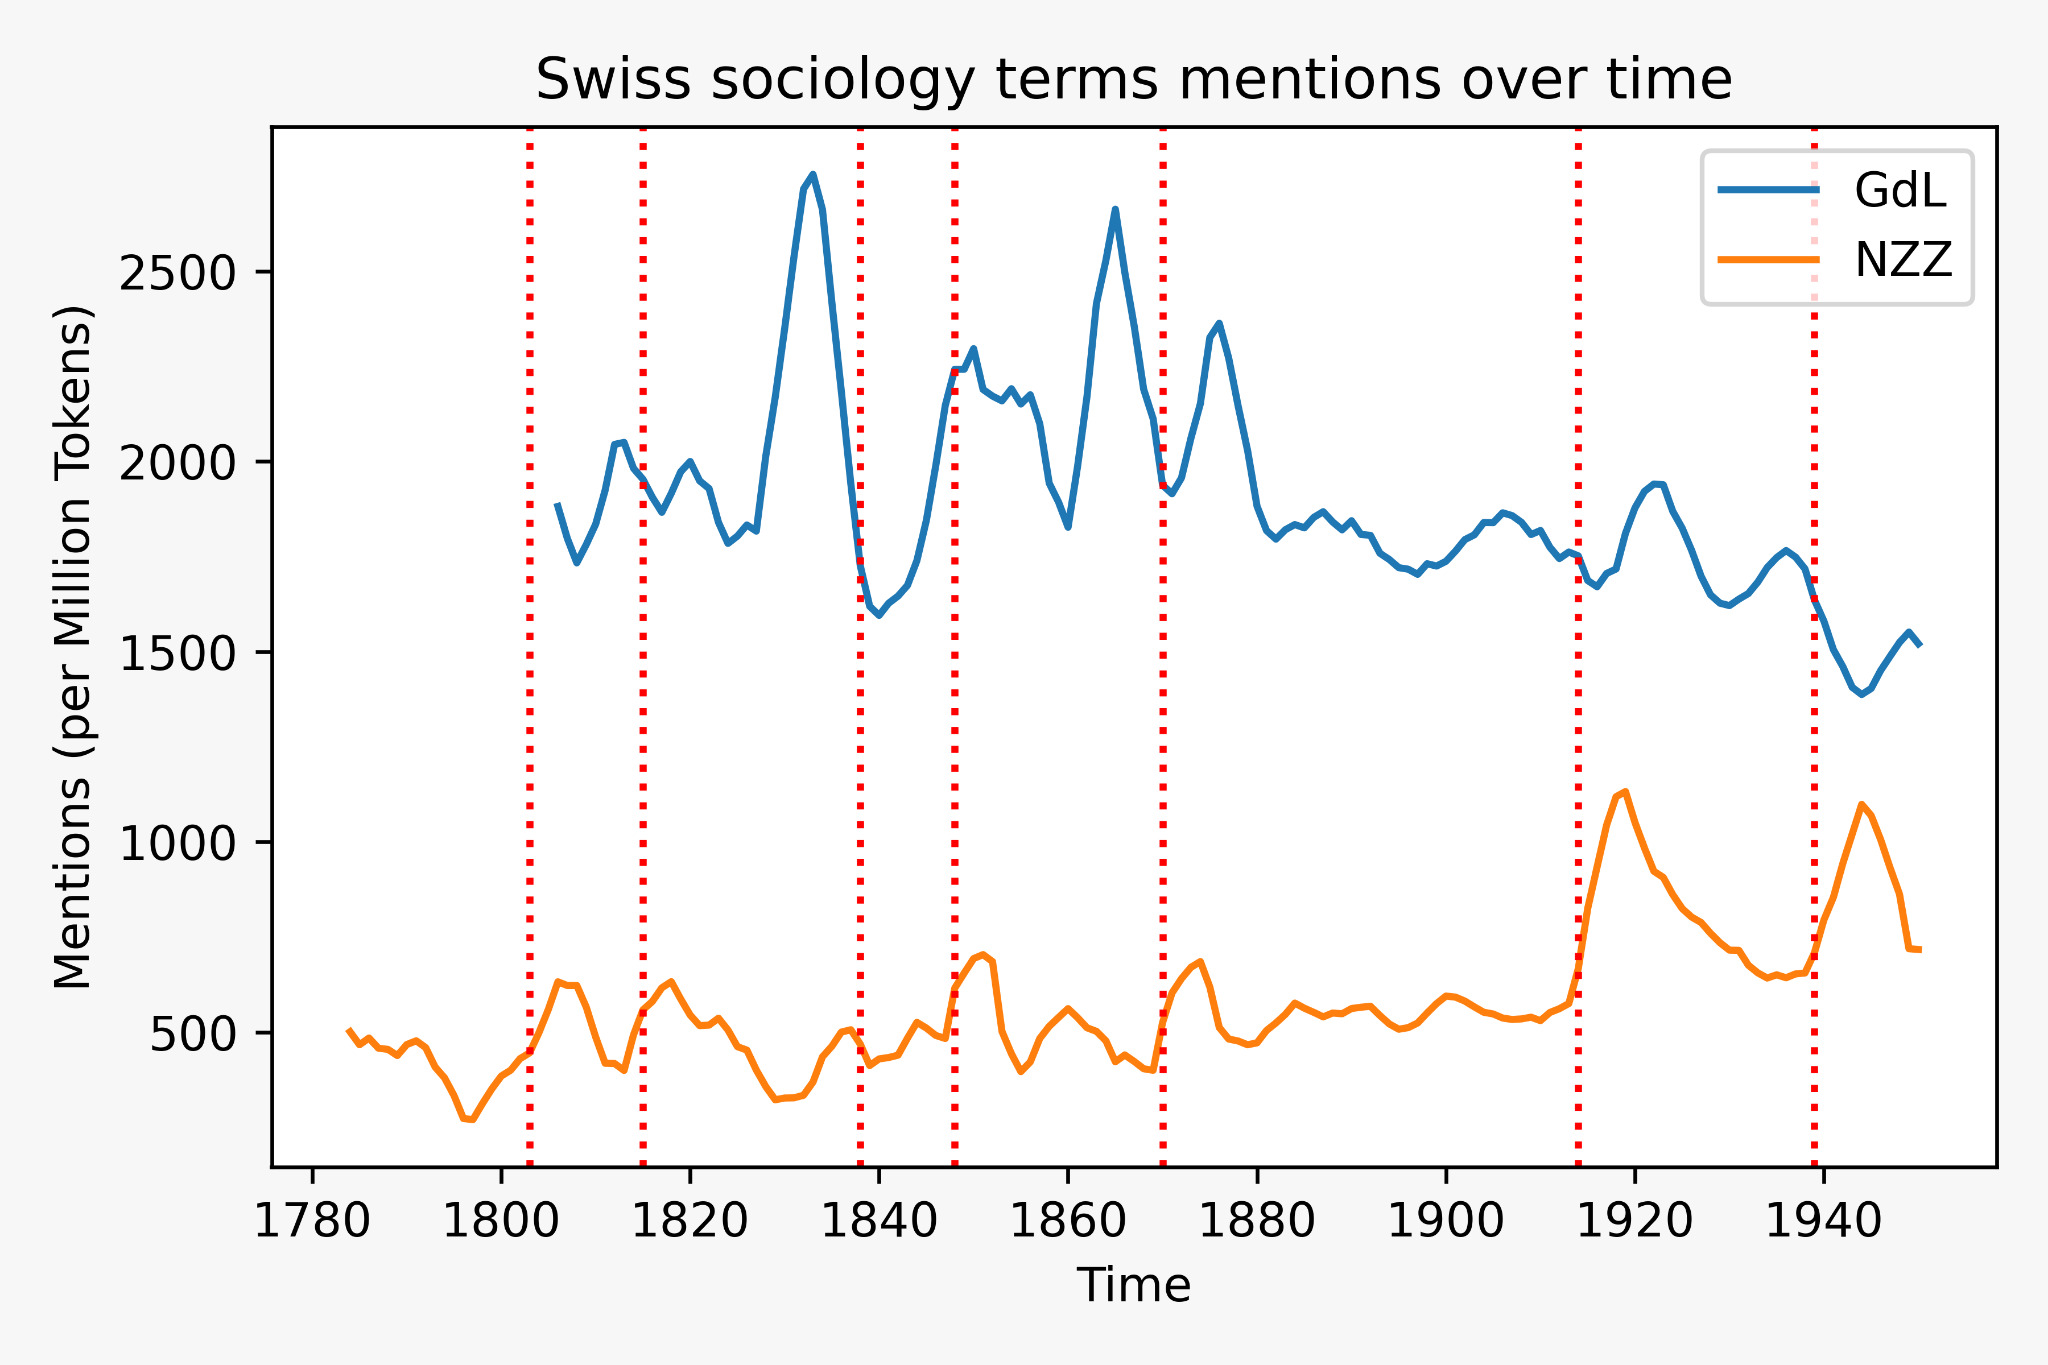
\includegraphics[width=1\linewidth]{figures/mentions_sociology.jpeg}
    \caption{Longitudinal analysis of cumulative frequencies of the 50 most popular TF-IDF tokens in the corpus. The frequencies are normalized per million tokens. The red lines represent the following important dates: Mediation under Napoleon (1803), Congress of Vienna (1815), Diplomatic conflict between Swiss confederacy and France (1838), Creation of modern Switzerland (1848), Creation of Italy and Germany (1870), Beginning of I. World War (1915), Beginning of II. World War (1939).}
    \label{fig:cumulative_sociology}
\end{figure}


\subsection{WWI Propaganda}
Considering that for the WWI propaganda extraction we used war vs non-war years newspapers, it's reasonable that all the factual information about the war will be present as the important tokens. Therefore, we did not take into account any terms which explicitly refer to military. The remaining terms were closely analysed in terms of their possible propaganda use. Finally, we decided to elaborate on three topics, which were frequent in the result TF-IDF scores, and important in terms of Swiss internal affairs during the wars. \par
The Red cross (tokens: croix rouge) is an organisation of great importance for the perception of the Swiss during the war conflicts, both in the foreign and internal relations. Its position and recognition was greatly increased during the first World War. Internally, the actions taken by the red cross could have been perceived as Swiss participation in the conflict, but not as an armed force but as a humanitarian power. It might have been an important fact for the population criticising the government for not taking any action during the major conflict. For external politics, the actions taken by red cross boosted the perception of Switzerland as a neutral country. \par

Swiss Neutrality (tokens: pays neutre, neutral staat, neutral land) is an important concept which was coined shortly before and during the I WW, was the key point of the Swiss political coherence during the major conflicts. The narration of opposition, the Swiss unlikeness, which allowed them to stay neutral (\emph{neutral staat}) while the continent was in the tragic conflict (\emph{kriegführend staat}), was a strongly integrating collaborative sentiment. 

Swiss Railways took an important role in country integration considering the hard travel conditions and the prior alienation of small mountain villages. The project, which was a great achievement both in terms of infrastructure and nation building, mainly took part in the XIX and beginning of XX century. It not only paved the way for fast information and ideas sharing through the country, but made a Swiss internal integration a much more convincing alternative to the cross-border integration, which could otherwise take place for each part of the Switzerland independently, decreasing the national coherence. \par

\begin{figure}[H]
    \centering
    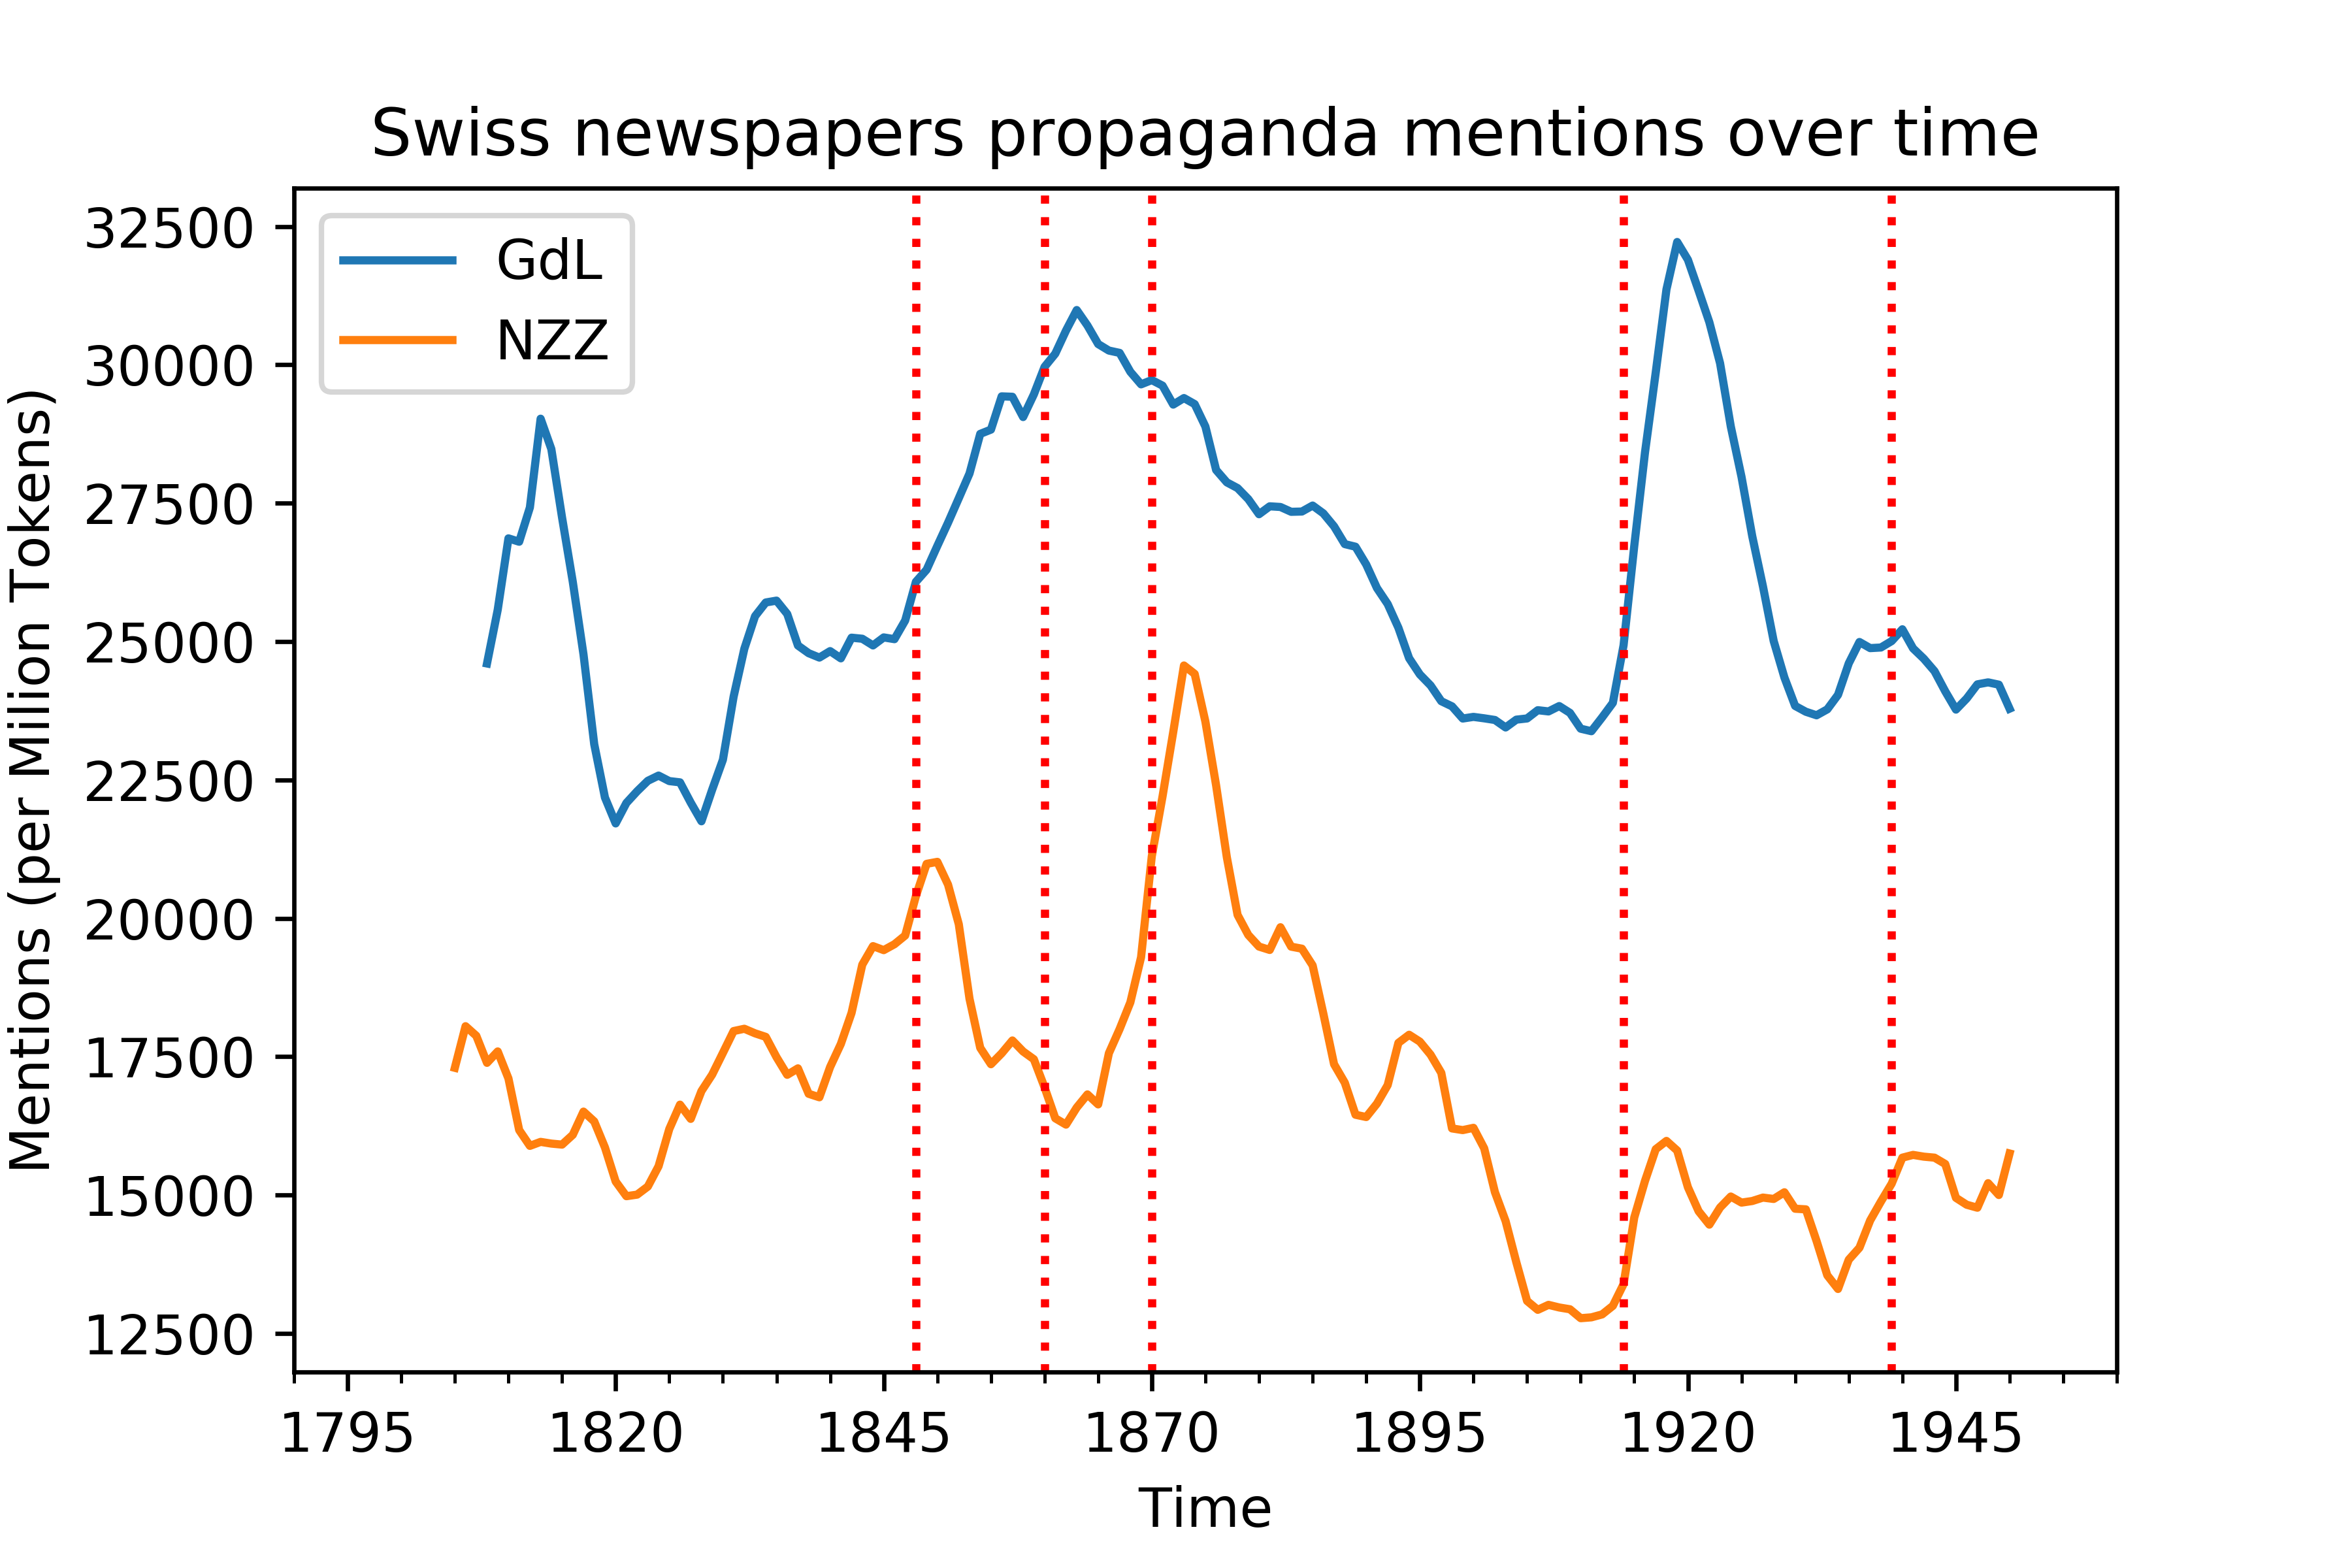
\includegraphics[width=1\linewidth]{figures_Michal/cumulative_propaganda.png}
    \caption{Longitudinal analysis of cumulative frequences of the most popular TF-IDF tokens in the corpus. The red lines represent important conflicts: Sonderbunden war, Savoy conflict, Franco-Prussian war, WWI, WWII}
    \label{fig:cumulative_propaganda}
\end{figure}

The detailed trend visible on Figure~\ref{fig:cumulative_propaganda}, alongside the detailed TF-IDF result tables, available in Appendix 6, provide some interesting insights into the Swiss newspapers propaganda. First, there is a visible trend of propaganda increase, consistent with the appearance of political situations dangerous for Swiss integrity. Secondly, while Franco-Prussian war and WWI remain of the highest importance, the other situations seem to be covered more locally only in the more involved part of Switzerland. Finally, we note nearly complete Swiss indifference to the WWII, which is surprising, but might be explained by the success of the WWI armed neutrality strategy and the wide consensus of Swiss public opinion, that the same strategy might work again.

\newpage

\section{Discussion \& Conclusions}
The extraction methods presented, the resulting sets of words depicting national identity and the final aggregated trends create a huge overhead in the results. A conclusion is therefore crucial and critical, and similarities and differences in the produced results need to be explained.\par
First, considering the resulting terms, different concepts and topics describing Swiss national identity have been detected within each obtained term list. Terms which encode locations or important historical protagonists constitute one of the topics that is common to all extractions. This, however, is rather unsurprising, thus discarded by this paper. A topic of interest is that which places Switzerland in relation with the international, relating Switzerland and neighbouring European powers. This topic is present in all three sources, although the precise functionality varies across the sources. In the historical sources, the surrounding powers seem to be the acting powers which force the Swiss cantons to build an alliance, which eventually would yield into a nation. The WWI propaganda shows a cemented nation resisting external forces. Lastly, the sociological papers depict Switzerland as influenced by its surrounding countries. The strong focus on external powers to define Swiss sentiment in all three sources clearly indicates that the definition of Swiss nationhood is bound discriminating between Swiss and non-Swiss.  \par
Moreover, the topic of Switzerland's neutrality and its military recur in all extractions. Its connotation varies again between the sources, however, parallels in its functionality can be found across all sources. First, the historical sources reflect on the importance of the Swiss military alliance and its resistance against outside powers. This narrative is continued by the WWI propaganda, which also strongly focuses on the Swiss neutrality and at last the sociological papers reflect on the cohesive powers of the common military service and shared experience of resistance as symbols for the construction of the identity.\par
A last, rather abstract topic, which is mainly covered by the historical and the political sources, describes political participation and institutions. Here the obtained terms seem to draw on two opposing concepts. One indicating that Swiss national identity is an invention of local elites and one that the Swiss nation is a deeply rooted in the the population, by a sort of collective awareness and memory. This reflects the discourse of Switzerland as both a voluntary nation (Willensnation) or a natural community (Wesensgemeinschaft) \citep{zimmer1999forging} introduced in the Research Context.\par

The time trends obtained by each term list partially mirror each other, but vary in magnitude and accentuation. It is visible that each source is a biased representation of its own time and thus yields higher trends during its respective time frame. However, the obtained time trends draw peaks in term mentions which coincide with significant historical events. Those historical events are either internal or external conflicts, which question or redefine the Swiss nation. It seems that during such events the investigated newspapers use a vocabulary which reflects or predetermines the terms which were computationally obtained. 
The usage of national identity defining words during times of internal or external conflict and restructuring might indicate that Swiss national identity still had to be solidified over the course of the XIX century. However, it seems that the peak indicating the beginning of the Second World is smaller and less significant in all three plots. This might signify that during the WWII Swiss nationalism was solidified to a point that less public discussion was necessary to convey Swiss national identity.

The overall picture of Swiss identity that was traced by this project can be summarized as follows: It is a process that is boosted by internal or external conflicts, by the need to define the Swiss from the non-Swiss. It is also a concept shaped by both political and cultural factors, by abstract and concrete ones. It relies on the symbols of military honors and sport ceremonies. It also relies on a common past rich of ideals of democracy, neutrality and driven by a strong patriotism.

However, this reconstruction is inherently limited and it is important to acknowledge its limitations. Firstly, the term extraction is largely biased in two directions: temporally and thematically. It is plausible that each source type resonates most with the language and events of the time the source was made, hence, there is an increase in frequency around the time of the sources. Furthermore, each of the sources depicts only a partial view on the nation, the first based on political-historical events, the second on demagogic myths and values and the last on abstract definitions of nationality. The already biased and lateral view of Swiss nation is further problematized by the inherent limitations of the TFIDF method, which can determine which words are rather specific to a document but cannot distinguish which words are more valuable than others. More specifically, the algorithm has no concept of the semantics of the words, thus, it cannot filter out infrequent words with very general meanings, or words that distance too much from the concept of nation. This limitation introduces also the need for vast manual filtering when analysing the extracted words. \par
Moving to the frequency time trends, properly normalizing the frequencies in time and across newspapers is complex. Although currently this paper normalizes by million tokens (so how many times a word appears every million tokens published in the newspaper in the specific year), this does not take into account the actual total number of articles in the year, nor in the Swiss region nor among a newspaper's specific edition. It does not indicate how relevant a word is to the unit of the article and it weighs too heavily when a word appears often in the same article. Moreover, when a peak is detected, it is difficult to separate when the mention is in reference to the Swiss case or to an international event. It is also difficult to understand whether the word extracted was used in the article with the same connotation it had when it was extracted. For instance, the XIX century can be mentioned in reference to the rise of Nationalism but also in various different contexts. Finally, the language barrier between the extraction for the French and the German corpora makes comparison between the two languages and corresponding trends almost impossible. \par

To overcome these limitations, ample future work is needed. A first step, which was partly tried in Appendix 7 is to investigate the context in which the words were used in the newspapers to check that they are actually used with the intended meaning and to better understand the modalities with which Swiss identity was treated. Another future step consists in extracting more similar words for the two languages, addressing the issues of translating between one and the other, either by using the same corpora for extraction or just translating the extracted words. An expansion to obviate the problems inherent to the method is to either expand the reference corpora to texts treating nationalism of other countries (but not Switzerland), to extract more 'Swiss' identity terms, and/or filter words using word embeddings and a distance measure from the concept of nationality. \par

Finally, we acknowledge that a complete analysis of the Swiss identity would require extending also to Romansh and Italian sources.

